\documentclass[english,12pt,letter]{article}

\usepackage{amsthm}
\usepackage[latin9]{inputenc}
\usepackage{babel}
\usepackage[hmargin=0.9in,vmargin=1.25in]{geometry}
\usepackage{graphicx}
\usepackage{subfigure}
\usepackage[colorlinks=true,citecolor=blue,urlcolor=blue]{hyperref}
\usepackage{amsmath}
\usepackage{amssymb,amsfonts}

\newtheorem{thm}{Theorem}
\newtheorem{lem}{Lemma}
\newtheorem{cor}{Corollary}
\newtheorem{dfn}{Definition}
\newtheorem{rmk}{Remark}

\newcommand{\Rnot}{\sigma_0}
\newcommand{\Sinf}{x_\infty}
\newcommand{\dom}{{\mathcal D}}
\newcommand{\R}{{\mathbb R}}
\newcommand{\xopt}{x_\text{opt}}
\newcommand{\yopt}{y_\text{opt}}
\newcommand{\ymax}{y_\text{max}}
\newcommand{\Dt}{\Delta t}
\newcommand{\Dx}{\Delta x}
\newcommand{\Dy}{\Delta y}

\DeclareMathOperator\supp{supp}

\begin{document}
\title{Optimal control of an SIR epidemic through finite-time non-pharmaceutical intervention}
\author{
  David I. Ketcheson\thanks{Computer, Electrical, and Mathematical Sciences \& Engineering Division,
King Abdullah University of Science and Technology, 4700 KAUST, Thuwal
23955, Saudi Arabia. (david.ketcheson@kaust.edu.sa)}
}
\maketitle

\abstract{
We consider the problem of controlling an SIR-model epidemic
by temporarily reducing the rate of contact within a population.
The control takes the form of a multiplicative reduction in the contact rate
of infectious individuals.  The control is allowed to be applied only over
a finite time interval, while the objective is to minimize the total number of
individuals infected in the long-time limit, subject to some cost function for
the control.  We first consider the no-cost scenario and analytically determine
the optimal control and solution.  We then study solutions when a cost of intervention
is included, as well as a cost associated with overwhelming the available medical resources.
Examples are studied through the numerical solution of the associated Hamilton-Jacobi-Bellman
equation.  Finally, we provide some examples related directly to the current pandemic.
}

\section{Problem description and assumptions}
The classical SIR model of Kermack \& Mckendrick \cite{kermack1927contribution} is
\begin{subequations} \label{SIR}
\begin{align} 
    x'(t) & = -\gamma \Rnot y(t) x(t) \label{eq:x} \\
    y'(t) & = \gamma \Rnot y(t) x(t) - \gamma y(t) \label{eq:y} \\
    (x(0),y(0)) & \in \dom := \{(x_0,y_0) : x_0 > 0, y_0 > 0, x_0+y_0 \le 1\},
\end{align}
\end{subequations}
where $x(t), y(t)$ represent the susceptible and infected populations
respectively, while the recovered population is $z(t)=1-x(t)-y(t)$.  The region
$\dom$ is forward-invariant and a unique solution exists for all time
\cite{hethcote2000mathematics}.  While
the temporal dynamics of \eqref{SIR} depend on both $\Rnot$ and $\gamma$, the set
of trajectories depends only on the basic reproduction number 
$\Rnot$.  Dynamics for two values of $\Rnot$ are
shown in Figure \ref{fig:dynamics}.  

The system \eqref{SIR} is at equilibrium if $y(t)=0$.  This equilibrium is stable if and
only if $x(t)\le 1/\Rnot$, a condition referred to as {\em herd immunity}.  If
this condition is not satisfied at
the initial time, then $y(t)$ will first increase until it is, and then decrease,
approaching zero asymptotically.  The SIR model assumes that recovery
confers permanent immunity.

\begin{figure}
    \centering
    \subfigure[$\sigma=3$]{\label{sigma3}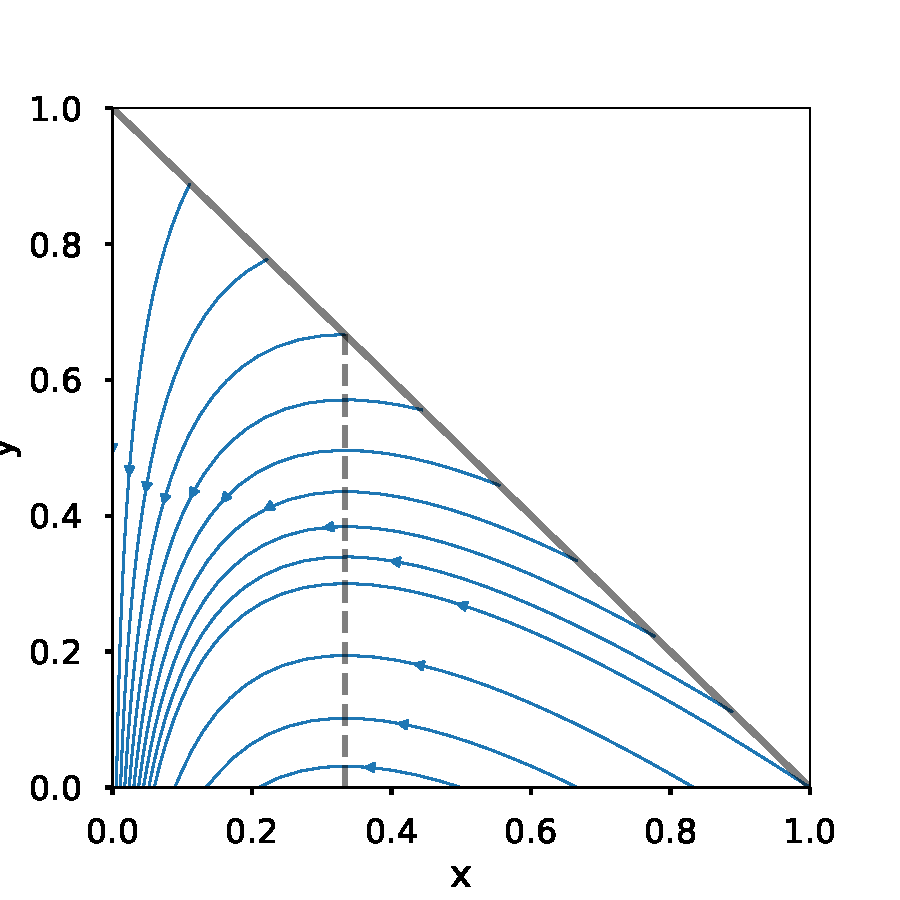
\includegraphics[width=0.49\textwidth]{figures/sigma3.pdf}}
    \subfigure[$\sigma=1.5$]{\label{sigma15}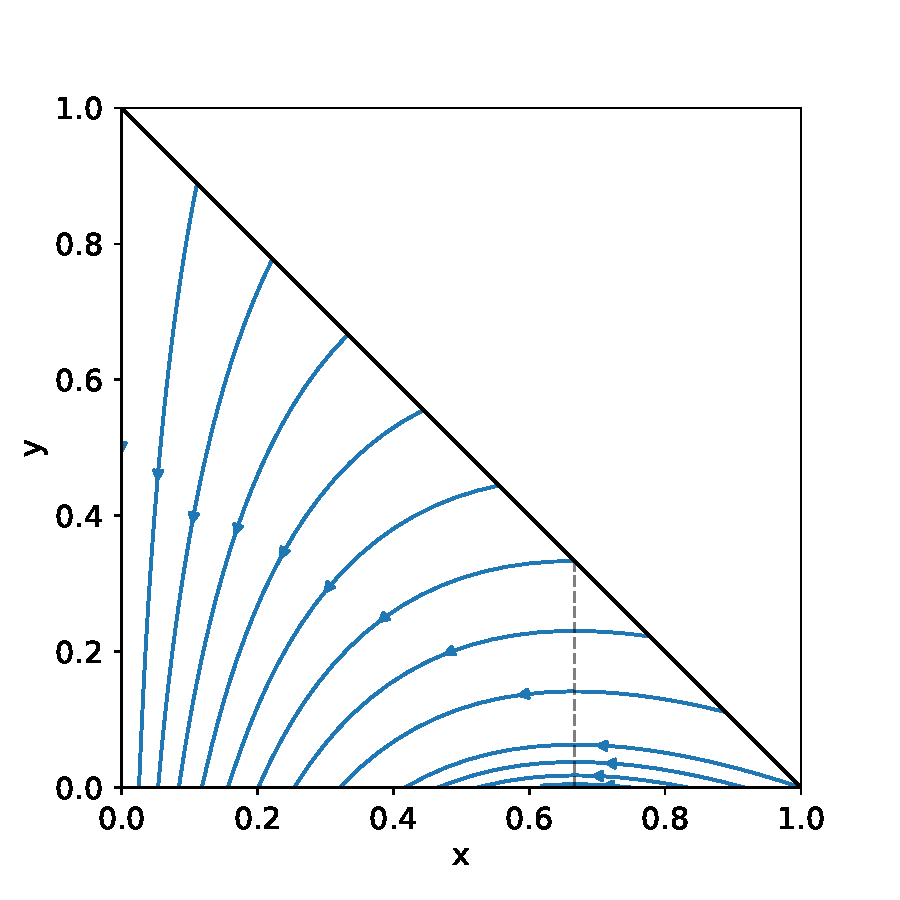
\includegraphics[width=0.49\textwidth]{figures/sigma15.pdf}}
    \caption{Dynamics of SIR model for two values of the basic reproduction number.
            The critical value $x=1/\sigma$ is shown with a dashed line.\label{fig:dynamics}}
\end{figure}

For many diseases affecting humans, herd immunity is achieved
through vaccination of a sufficient portion of the population.  Herein
we assume a vaccine is unavailable, so that herd immunity can only be achieved
through infection and recovery.
Our goal is to minimize $z_\infty := \lim_{t \to \infty} z(t)$, or equivalently
(since $y_\infty=0$)
to maximize the long-time limit of the susceptible fraction:
$\Sinf = \lim_{t\to\infty} x(t)$.
This has the effect of minimizing
the number of eventual deaths, which would be proportional to $z_\infty$.

This is equivalent to minimizing the number of deaths, if we assume that
some fixed fraction of the recovered population $z(t)$ dies from the disease.
From the foregoing it is clear that $\Sinf \le 1/\Rnot$.  The difference
$1/\Rnot-\Sinf$ is referred to as {\em epidemiological overshoot}.
For COVID-19, a review of early estimates of $\Rnot$ can be found in
\cite[Table 1]{liu2020reproductive}, with mean 3.28 and median 2.79.
In accordance with these estimates, we use a value $\Rnot=3$ in most of
the examples in this work.  With this value, the SIR model implies that eventually
at least two-thirds of the world population will eventually have COVID-19 antibodies;
this number is likely to be significantly higher in reality due to epidemiological
overshoot.  For instance, it can be seen from Figure \ref{sigma3} that, starting
from a fully susceptible population and a small number of infected individuals,
in the absence of control the SIR model predicts that over $90\%$ of the population
would be infected.

This overshoot can in principle be reduced through
non-pharmaceutical intervention (NPI), which is simply a means to
reduce contact between infected and susceptible individuals.  We model a NPI
control via a time-dependent reproduction number $\sigma(t)\in[0,\Rnot]$ with the system
\begin{subequations} \label{SIRq}
\begin{align}
    x'(t) & = -\gamma \sigma(t) y x \\
    y'(t) & = \gamma \sigma(t) y x - \gamma y \\
    (x(0),y(0)) & \in \dom := \{(x_0,y_0) : x_0 > 0, y_0 > 0, x_0+y_0 \le 1\}.
\end{align}
\end{subequations}
A temporary reduction in $\sigma$ can account for both
population-wide interventions and interventions specific to identified infectious
(or possibly infectious) individuals.  The SIR model with a time-dependent
reproduction number (or equivalently, a time-dependent contact rate) has been 
considered before, for instance in \cite{sun2020tracking}.

Typically, an epidemic does not result in substantial {\em permanent} change in the contact rate of
a population.  We therefore assume 
\begin{align} \label{q-shortterm}
    \sigma(t)=\Rnot \text{ for } t>T,
\end{align}
i.e., that intervention can only be applied over a finite interval $t \in [0,T]$.
Since $x_\infty=1/\sigma_0$ only at the single point $(x=1/\sigma_0,y=0)$, and since 
the $y=0$ axis cannot be reached in a finite time, \eqref{q-shortterm} implies
that any solution must have $x_\infty<1/\sigma_0$.
%In either model \eqref{SIR} or \eqref{SIRq}, the zero-infection axis
%$y=0$ can only be reached after an infinite amount of time. Therefore our
%objective will be to achieve $x_\infty=1/\sigma_0 - \epsilon$ for a prescribed
%value $\epsilon$.

We state the control problem as follows:
\begin{align} \label{eq:inf-time-problem}
\begin{aligned}
& \text{Given } (x_0, y_0)\in\dom, \sigma_0>0, T>0,  \\
& \text{ choose an admissible control } \sigma(t): [0,T] \to [0,\Rnot] \text{ to minimize }  \\
&     J(x(t),y(t),\sigma(t)) = -\lim_{t\to\infty} x(t) + \int_0^T L(x(t),y(t),\sigma(t)) dt \\
& \text{ subject to } \eqref{SIRq}.
\end{aligned}
\end{align}
Here $J$ is the objective function that accounts for the desire to
minimize infections as well as a running cost of imposing control.


There is a large body of work on compartmental epidemiological models
and control for such models; see e.g. \cite{hethcote2000mathematics,lenhart2007optimal}
and references therein.  A number of works focus on optimal control
through vaccination; see e.g. \cite{kar2011stability}.
Other works, such as \cite{yan2008optimal,safi2013dynamics,agusto2013optimal}
focus on explicit modeling of and/or control through quarantined and isolated individuals.
A review of work on optimal control in compartmental epidemiological models is
presented in \cite{sharomi2017optimal},
along with the formulation of necessary conditions (based on
Pontryagin's maximum principle) for various extensions of the SIR model.
For modeling and control based on even more detailed models incorporating
spatial spread and human networks, see e.g. \cite{ferguson2005strategies}.

\subsection{Objectives and contributions}

The modeling and assumptions in the present work are motivated by the
current COVID-19 epidemic, which so far is being managed through broad
NPIs and without a vaccine.  In order to understand the effects of NPIs
imposed on an entire population, we stick to the simple model \eqref{SIRq}
rather than explicitly modeling quarantined individuals.
Since such population-wide measures cannot be maintained indefinitely, we
invoke the finite-time control assumption \eqref{q-shortterm}.
This assumption is not new (see e.g. \cite{greenhalgh1988some}),
but unlike previous works our objective function is still based on the
long-term outcome (rather than the outcome at time $T$).
This drastically changes the nature of optimal solutions.
%In the last section of this work we also consider the goal of avoiding
%hospital overflow (through {\em flattening the curve}).

Although the broad motivation for this work comes from the current epidemic,
our primary objective is to understand general properties of optimal controls
for the variable-$\sigma$ SIR system \eqref{SIRq}.  To this end, we also
investigate solutions in certain
asymptotic regimes (such as when there is little or no cost associated
with the control).  Nevertheless, the values of the key parameters $\gamma$
and $\Rnot$ for all examples are chosen to fall in the range of current estimates for
COVID-19.

One novel aspect of this work is that the problem is posed in terms of the
infinite-time limit, but formulated in a way that only requires solution
over a finite time interval.  Indeed, without this reformulation we found
that the problem was extremely ill-conditioned; this reformulation is also
needed in order to compute approximate solutions via a Hamilton-Jacobi-Belmman
equation.
This reformulation is presented in Section \ref{sec:prelims}.  The main theoretical
result is an exact characterization of the optimal control when $L=0$, given
as Theorem \ref{thm:no-cost} in Section \ref{sec:analytic}.  

Typical results in the literature on control of compartmental epidemiological models
are numerical and are based on Pontryagin's weak maximum principle, which gives only
necessary conditions for optimality.  At best, uniqueness is shown for small times; see e.g. 
\cite{kirschner1997optimal,fister1998optimizing,jung2002optimal,yan2008optimal,kar2011stability}.
In contrast, here the main result includes a proof of optimality for arbitrarily large times.
In Section \ref{sec:exploration} we explore
the behavior of optimal solutions for $L\ne 0$ under various interesting
cost functions and parameter regimes.  Here the results are based on
solutions of the relevant Hamilton-Jacobi-Bellman equation, which is
both necessary and sufficient for optimality.
In Section \ref{sec:application} we consider direct application to the COVID-19
pandemic.  Some conclusions are drawn in Section \ref{sec:conclusion}.

\section{Formulation over a finite time interval\label{sec:prelims}}
In this section we reformulate the control problem \eqref{eq:inf-time-problem} in terms of
the solution over a finite time interval $[0,T]$.  This reformulation is
necessary both to facilitate the exact solution in Section \ref{sec:analytic}
and to arrive at a numerically-tractable problem for computing
approximate solutions, as described in Section \ref{sec:exploration}.

%\subsection{Notation}
%The control above is given as $q(t)$, but for most purposes it is more
%convenient to work with the effective reproduction number, defined as
%$$
%    \sigma(t) := (1-q(t))\Rnot = (1-q(t))\beta/\gamma.
%$$
%We will often simply refer to $\sigma(t)$ as the control.

In general, the solution of \eqref{SIRq} depends on the initial data
$(x_0,y_0)$, the control $\sigma(t)$, and time $t$, so it is natural to write
$x(t;\sigma(t),x_0,y_0)$.
In what follows it will be convenient to make a slight abuse of notation and
write $x(t;\sigma(t))$ or $x(t)$ when there is no chance of confusion.

For a fixed reproduction number, the asymptotic susceptible fraction $\Sinf$
can be obtained from the solution $x(t), y(t)$ at any time $t$, since solutions
of \eqref{SIR} move along contours of $\Sinf$.  Thus we will write $\Sinf(x,y)$
or $\Sinf(x,y,\Rnot)$.

\subsection{A formula for $\Sinf$}
In this subsection we review the solution of the SIR model without
control \eqref{SIR}.
It can be shown that $x(t)$ satisfies (see \cite{harko2014exact,pakes2015lambert} and
\cite[pp.707-708]{kermack1927contribution})
$$
    x(t)e^{\Rnot z(t)} = x_0 e^{\Rnot z_0}.
$$
Since $z=1-x-y$ we define
$$
   \mu(x,y,\Rnot) := x(t) e^{-\Rnot(x(t)+y(t))},
$$
which is constant in time for any solution of \eqref{SIR}.
The trajectories in Figure \ref{fig:dynamics} are thus also contours of $\mu$.
Since $y_\infty=0$, we have
$$
    x_\infty = x_0 e^{\Rnot(x_\infty-x_0-y_0)} = \mu(x_0,y_0,\Rnot) e^{\Rnot x_\infty}.
$$
Setting $w=-x_\infty \Rnot$ we have
$$
    we^w = -x_0 \Rnot e^{-\Rnot(x_0+y_0)} = -\mu \Rnot.
$$
Thus $w = W_0(-\mu\Rnot)$ where $W_0$ is the principal branch of Lambert's $W$-function \cite{pakes2015lambert},
and
\begin{align} \label{eq:xinf}
    x_\infty(x,y,\sigma_0) = -\frac{1}{\Rnot}W_0(-\mu(x,y,\sigma_0) \Rnot).
\end{align}
Formula \eqref{eq:xinf} allows us to rewrite the problem \eqref{eq:inf-time-problem} in
terms of the state at time $T<\infty$:
\begin{align} \label{eq:basic-problem}
\begin{aligned}
& \text{Given } (x_0, y_0) \in \dom, \sigma_0>0, T>0,  \\
& \text{ choose an admissible control } \sigma(t): [0,T] \to [0,\Rnot] \text{ to minimize }  \\
&     J = -x_\infty(x(T),y(T),\sigma_0) + \int_0^T L(\sigma(t) dt \\
& \text{ subject to } \eqref{SIRq}.
\end{aligned}
\end{align}

In what follows we will also require the derivatives of $\Sinf$ with respect to $x$, $y$, and $\mu$.
Direct computation gives
\begin{subequations} \label{xinf-grad}
\begin{align}
    \frac{\partial \Sinf}{\partial y(t)} & = -\frac{\Rnot \Sinf}{1-\Rnot \Sinf} \\
    \frac{\partial \Sinf}{\partial x(t)} & = \left(1-\frac{1}{x(t)\Rnot}\right) \frac{\partial \Sinf}{\partial y(t)}
      = \frac{1-\Rnot x(t)}{1-\Rnot \Sinf} \cdot \frac{\Sinf}{x(t)} \\
    \frac{\partial \Sinf}{\partial \mu} & = \frac{e^{\Rnot\Sinf}}{1-\Rnot \Sinf}.
\end{align}
\end{subequations}
Using these expressions we can also compute the rate of change of $\Sinf$ when some
control $\sigma(t)$ is applied:
\begin{align} \label{dxinf-dt}
    \frac{\partial \Sinf}{\partial t} = \frac{\gamma y \Sinf}{1-\Rnot\Sinf}(\Rnot - \sigma(t)).
\end{align}
From this we see that the impact of an intervention on $\Sinf$ is independent of $x(t)$ and
directly proportional to $y(t)$.  This indicates that intervention is more impactful
when there is a larger infected population.
%\begin{align*}
%\frac{d \Sinf}{d\mu} = W'(-\mu \Rnot) = \frac{1}{e^{-\Rnot\Sinf}-\mu \Rnot} > 0,
%\end{align*}
%so $\Sinf$ is a monotone function of $\mu$ and maximizing the former is equivalent to
%maximizing the latter.
%Now
%\begin{align*}
%    \frac{d}{dt} \mu(x(t;\sigma(t)),y(t;\sigma(t)),\Rnot) = (\Rnot-\sigma(t))\gamma y(t;\sigma(t)) \mu(t).
%\end{align*}
%\begin{align*}
%    \frac{\partial \Sinf}{\partial y} & = W'(-\mu\Rnot) \frac{\partial \mu}{\partial y}
%\end{align*}
%
%
%The formulas in this section also hold for the solution of \eqref{SIRq} if
%$q(t)$ is a constant function and $\Rnot$ is replaced in these formulas by
%$\sigma=(1-q)\Rnot$.


%We define the solution operator $\phi_t(\beta,\gamma): \dom \to \dom$ as the map
%that takes an initial condition $(x_0,y_0)$ to the solution $(x(t),y(t))$
%via the solution of \eqref{SIR}.  We further define for $u\in\dom$
%$$
%    x_\infty(u,\sigma) = \lim_{t\to\infty} \phi_t(\sigma,1)u.
%$$
%Observe that each trajectory in Figure \ref{fig:dynamics} is a contour of $x_\infty$.
%Our objective then is to minimize $x_\infty((x(T),y(T)),\Rnot)$.

\subsection{Bounds on $\Sinf$}
Now we turn our attention to the SIR system with control \eqref{SIRq}.

\begin{dfn} ({\bf Admissible control})
Given a basic reproduction number $\Rnot$, we say a control fuction $\sigma(t)$ is
admissible if it is piecewise continuous and $0\le \sigma(t) \le \sigma_0$ for all $t$.
\end{dfn}

It is straightforward to show that \eqref{SIRq} has a unique solution for all time
for any initial data in $\dom$ and any admissible control, by the same
arguments used for \eqref{SIR}.
%By applying the control we can move the solution to a different contour of
%$x_\infty(\cdot,\sigma)$.  
The proof of the next lemma shows that applying any control $\sigma(t)<\Rnot$ over
any length of time leads to an increase in $x_\infty$.
\begin{lem}
Let $\Rnot>0$ and $(x_0,y_0)\in\dom$ be given. % and define $X_\infty = x_\infty(x_0,y_0,\Rnot)$.
Let $\sigma(t)$ be an admissible control.  Then for $t\ge0$ we have
$$
    x_\infty(x(t;\sigma(t)),y(t;\sigma(t)),\Rnot) \ge x_\infty(x_0,y_0,\Rnot).
$$
\end{lem}
\begin{proof}
    Dividing \eqref{eq:y} by \eqref{eq:x} gives
    \begin{align} \label{eq:dydx}
        \frac{dy}{dx} = -1 + \frac{1}{\sigma(t) x}.
    \end{align}
    Thus reducing $\sigma(t)$ has the effect of increasing $dy/dx$.
    Since all trajectories flow to the left ($x$ is a decreasing function of $t$),
    this means that the solution trajectory obtained with $\sigma(t)$ lies
    below that obtained with $\sigma_0$, for all $t>0$.  Since
    $\Sinf$ is a decreasing function of $y$, this completes the proof.
\end{proof}

Thus for any admissible control and any initial data we have
$$
\Sinf(x_0,y_0,\Rnot) \le \Sinf(x(T),y(T),\Rnot) \le 1/\Rnot.
$$

\subsection{Formulation as a boundary value problem\label{sec:pmp}}
Standard application of Pontryagin's maximum principle gives necessary conditions
for a solution of \eqref{eq:basic-problem}.  The Hamiltonian for this problem is
\begin{align} \label{eq:ham}
    H(x(t),y(t), \sigma(t), \lambda_{1,2}(t), t) = -\lambda_1(t) \gamma \sigma(t) y(t) x(t) + \lambda_2(t)\gamma y(t)(\sigma(t) x(t) - 1) + L(x(t),y(t),\sigma(t)),
\end{align}
and the adjoint variables are defined by
%Let $\sigma^*(t)$ denote an optimal control for \eqref{eq:basic-problem}.  Then we
%define functions $\lambda_{1,2}(t)$ via
\begin{subequations}\label{lambda-odes}
\begin{align} 
    \lambda_1'(t) & = -\frac{\partial H}{\partial x} = (\lambda_1-\lambda_2)\gamma\sigma(t) y(t) - \frac{\partial L}{\partial x} \\
    \lambda_2'(t) & = -\frac{\partial H}{\partial y} = (\lambda_1-\lambda_2)\gamma\sigma(t) x(t) + \lambda_2 \gamma - \frac{\partial L}{\partial y} \\
    \lambda_2(T) & = -\frac{\partial \Sinf(T)}{\partial x} = \frac{\partial }{\partial y(T)} (-x_\infty(x(T),y(T),\Rnot) \\
    \lambda_1(T) & = -\frac{\partial \Sinf(T)}{\partial y} =\frac{\partial }{\partial x(T)} (-x_\infty(x(T),y(T),\Rnot) = \left(1-\frac{1}{x(T)\Rnot}\right)\lambda_2(T),
\end{align}
\end{subequations}
where $x(t), y(t)$ satisfy $\eqref{SIRq}$.
The final conditions for $\lambda_{1,2}$ can be computed from \eqref{xinf-grad}.

\begin{thm}
    Let $(x_0, y_0)\in\dom$ and $\Rnot, \gamma, T\ge 0$ be given.  If $\sigma^*(t)$ is an optimal
    control for \eqref{eq:basic-problem} and $(x^*(t),y^*(t))$ are the corresponding optimal
    trajectory, then there exist functions
    $\lambda_{1,2}(t)$ satisfying \eqref{lambda-odes} with $x(t)=x^*(t), y(t)=y^*(t)$, and
    \begin{align} \label{eq:sigma-c2}
        \sigma^*(t) = \max\left(0,\min\left(\sigma_0,\hat{\sigma}(t)\right)\right),
    \end{align}
    where
    \begin{align} \label{eq:dldsig}
        \left. \frac{\partial L}{\partial \sigma}\right|_{\sigma(t)=\hat{\sigma}(t)} = - (\lambda_2(t)-\lambda_1(t))\gamma y x.
    \end{align}
\end{thm}
\begin{proof}
    This is a consequence of the weak Pontryagin's maximum principle; the condition \eqref{eq:dldsig}
    comes from requiring $\partial H/\partial \sigma = 0$.
\end{proof}


\subsection{Infinite-time control}
In this section only, we consider controls that reach the optimal value $\Sinf = 1/\Rnot$.
This is achieved only at $(x,y)=(1/\Rnot,0)$, a state that cannot be reached
from any other state without imposing some control, and which in any case can
only be reached after an infinite time.  Thus we momentarily set aside the restriction
\eqref{q-shortterm} and consider controls over the semi-infinite interval $t\in[0,\infty)$.
We assume that $x_0\ge1/\Rnot$, since otherwise the maximum achievable value of $\Sinf$
is $x_0$, which would be achieved by taking simply $\sigma(t)=0$ for all $t$.
We also take $L=0$ so that an optimal control is any control satisfying
$$
    \lim_{t \to \infty} x(t,\sigma(t)) = 1/\Rnot.
$$
There are infinitely many such controls.  Two are particularly simple and
are of interest.

The first is a constant control $\sigma(t) = \sigma_*(x_0, y_0, \Rnot)$.
By \eqref{eq:xinf} we must have $\Sinf(x_0,y_0,\sigma_*)=1/\Rnot$, so $\sigma_*$ is the solution of
$$
    W_0(-\mu(x_0,y_0,\sigma_*)\sigma_*) = -\frac{\sigma_*}{\sigma_0}.
$$

The second is a bang-bang control in which
$$
    \sigma(t) = \begin{cases} \Rnot & x>1/\Rnot \\ 0 & x=\Rnot. \end{cases}
$$
The response for each of these controls is shown for a specific example in
Figure \ref{fig:two-controls}.
\begin{figure}
    \centering
    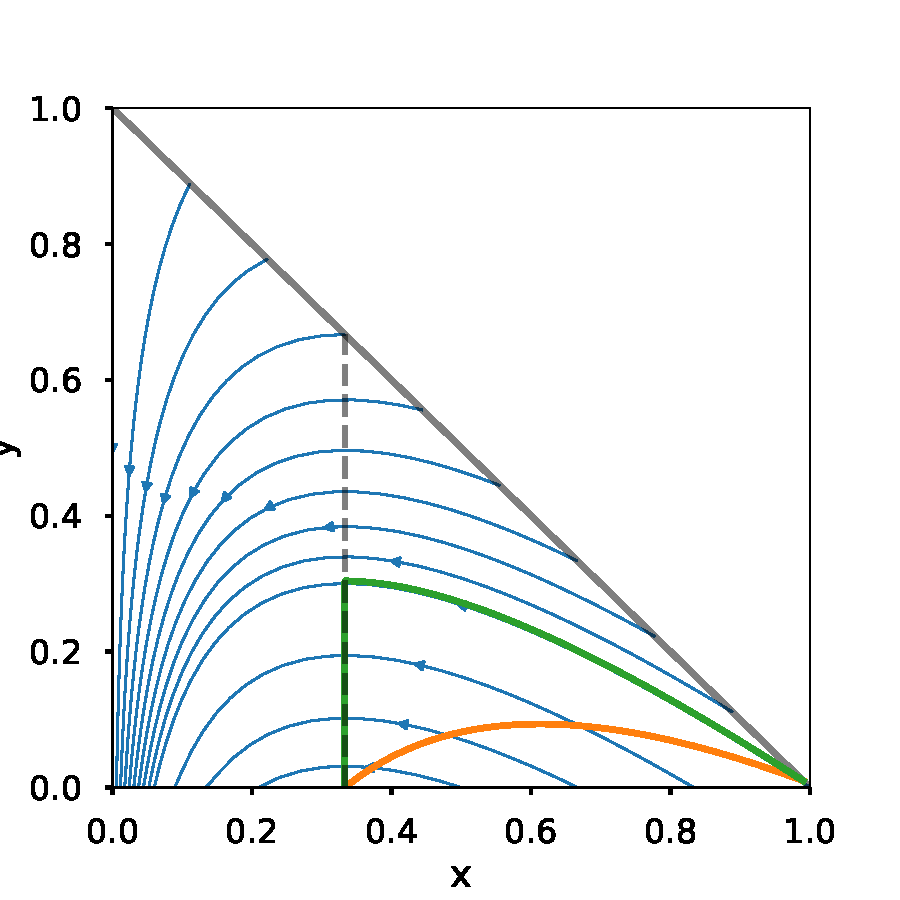
\includegraphics[width=0.5\textwidth]{figures/twocontrols.pdf}
    \caption{Two infinite-time controls that give $\Sinf=1/\Rnot$.  Here $\Rnot=3$ and
        $(x_0,y_0)=(0.99,0.01)$.  For the constant control, $\sigma(t)=\sigma_*\approx(1-0.4557)\Rnot$.\label{fig:two-controls}}
\end{figure}



\section{Optimal control with $L=0$\label{sec:analytic}}
In this section we derive the exact solution of the control problem
\eqref{eq:basic-problem} with $L=0$ (i.e., when the goal of increasing $x_\infty$ completely
trumps any associated costs or other concerns).  Then \eqref{eq:basic-problem} becomes
\begin{align} \label{eq:no-cost-problem}
\begin{aligned}
& \text{Given } (x_0, y_0)\in \dom, \sigma_0>0, T>0, \\
& \text{ choose an admissible control } \sigma(t): [0,T] \to [0,\Rnot] \\
& \text{ to minimize }  J = -x_\infty(x(T),y(T),\sigma_0) \\
& \text{ subject to } \eqref{SIRq}.
\end{aligned}
\end{align}
This problem can be reformulated as a minimum-time control problem.  

\begin{lem} \label{lem:min-time}
Let $\sigma^*(t)$ be an optimal control for \eqref{eq:no-cost-problem}, and
let $(x^*(T),y^*(T))$ denote the corresponding terminal state.
Then there is no admissible control that reaches $(x^*(T),y^*(T))$ from $(x_0,y_0)$
before time $T$.
\end{lem}
\begin{proof}
Suppose there were a control $\hat{\sigma}(t)$ that leads to $(x(t^*),y(t^*)) = (x^*(T),y^*(T))$ for some $t^*<T$.  Then
we could obtain a smaller value of $J$ in \eqref{eq:no-cost-problem} by using
$\hat{\sigma}$ up to time $t^*$ combined with the choice $\sigma(t)=0$ for $t>t^*$.
This contradicts the optimality of $\sigma^*(t)$.
\end{proof}

Furthermore, the optimal control must be a bang-bang control.
\begin{lem} \label{lem:bang-bang}
Let $\sigma(t)$ be an optimal control for \eqref{eq:no-cost-problem}.
Then
\begin{align} \label{eq:switch}
    \sigma(t) & = \begin{cases} 0 & \lambda_1(t)<\lambda_2(t) \\ \sigma_0 & \lambda_1(t) > \lambda_2(t) \end{cases}
\end{align}
where $\lambda_{1,2}(t)$ are given by \eqref{lambda-odes}.
\end{lem}
\begin{proof}
From \eqref{eq:ham} with $L=0$, we have
$$
\frac{\partial H}{\partial \sigma} = (\lambda_2(t)-\lambda_1(t))\gamma y(t) x(t).
$$
The optimality condition then implies \eqref{eq:switch} except at points where $\partial H/\partial \sigma=0$
(see e.g. \cite[Ch. 17]{lenhart2007optimal}.
Since $x(t),y(t) >0$ for $t<\infty$, we have that $\partial H/\partial \sigma=0$
if and only if $\lambda_1=\lambda_2$.  Suppose that the latter condition holds on
an open interval.  By \eqref{lambda-odes}, that would imply that $\lambda_1'(t) = \lambda_2'(t)=0$ on this
interval and hence for all $t$, which contradicts the boundary conditions \eqref{lambda-odes}.
\end{proof}

This motivates the following lemma.

\begin{lem} \label{lem:shortest-path}
Let $(x_0,y_0)$ and $(x_1,y_1)$ be given such that $x_0, x_1 \ge 1/\Rnot$ and
$\Sinf(x_0,y_0,\Rnot)\ge\Sinf(x_1,y_1,\Rnot)$.
Let $\sigma(t)$ be a bang-bang control such that $(x(t_1;x_0,y_0,\sigma(t)),y(t_1;x_0,y_0,\sigma(t)))=(x_1,y_1)$
for some $t_1\ge0$.  Then the minimum value of $t_1$ is achieved by taking
\begin{align} \label{eq:one-switch}
    \sigma(t) & = \begin{cases}
        \Rnot & t<t^* \\
        0 & t^* \le  t \le t_1,
    \end{cases}
\end{align}
where $t^*$ satisfies $x(t^*;x_0,y_0,\Rnot)=x_1$.
\end{lem}
\begin{proof}
Since $\sigma(t)$ is a bang-bang control, the trajectory $(x(t;\sigma(t)),y(t;\sigma(t)))$ 
consists of a sequence of segments each of which is a solution of
\eqref{SIRq} with $\sigma=0$ (traveling directly downward) or with $\sigma=\sigma_0$
(traveling along a contour of $x_\infty$).  Some trajectories of this type are
illustrated in Figure \ref{fig:bangbangtraj}.  Notice that each trajectory must
traverse the same distance in the x-direction; since $x'(t)=-\beta xy$ this
travel is faster at larger $y$ values.  Meanwhile, the total length of all the
downward ($\sigma=0$) segments is the same for any trajectory, and since for
these segments $y'(t) = -\gamma y$, travel is again faster at larger $y$ values.
The control given in the lemma makes all these traversals at the largest
possible values of $y$, so it arrives in the shortest time.
\end{proof}

Combining these three lemmas, we obtain the following.
\begin{thm} \label{thm:one-switch}
    Any optimal control for \eqref{eq:no-cost-problem} is of the form \eqref{eq:one-switch}
    with $t_1=T$.
\end{thm}
\begin{proof}
    By Lemmas \ref{lem:min-time} and \ref{lem:bang-bang}, the optimal control must be bang-bang and must solve
    the optimal-time problem.  Then Lemma \ref{lem:shortest-path} applies and gives the stated result.
\end{proof}

\begin{figure}
    \centering
    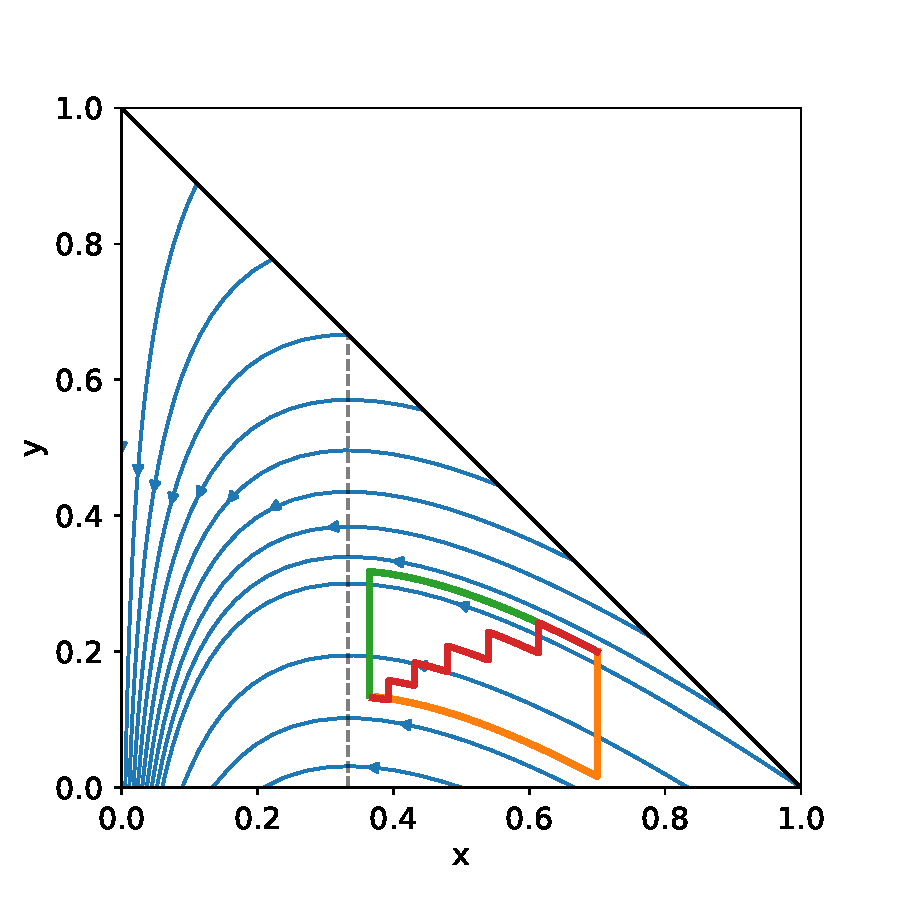
\includegraphics[width=0.5\textwidth]{figures/threepaths.pdf}
    \caption{Three different paths between two states, each obtained
    with a bang-bang control.  The top (green) path arrives in the shortest time.\label{fig:bangbangtraj}}
\end{figure}
%The lemma above holds for the set of all admissible controls, but here we
%only need the result for bang-bang controls.
We can now give the solution of \eqref{eq:no-cost-problem}.
\begin{thm} \label{thm:no-cost}
The optimal control for \eqref{eq:no-cost-problem} is unique and is given by
\begin{align}
    \sigma(t) & = \begin{cases}  
        \Rnot & t<t^* \\
        0 & t^* \le  t \le T,
    \end{cases}
\end{align}
where 
\begin{align} \label{eq:dropcond}
    t^*=0 \text{ if } x_0\le\frac{1}{\sigma_0(1-e^{-\gamma T})},
\end{align}
and otherwise $t^*$ is the unique solution of
\begin{align} \label{xtstar}
    x(t^*;\Rnot,x_0,y_0) = \frac{1}{\sigma_0(1-e^{-\gamma(T-t^*)})}.
\end{align}
\end{thm}
\begin{proof}
First, suppose $x(0)\le1/\sigma_0$.  The claimed optimal control gives $x(T)=x_0$, whereas
any other control will give $x(T)<x_0$.  Similarly, we see from \eqref{SIRq} that
the optimal control gives $y(T)=e^{-\gamma T}y_0$ and any other control will
lead to a larger value of $y(T)$.  Since $\Sinf$ is a decreasing function of $y$ and
(for $x<1/\Rnot$) an increasing function of $x$, the proposed control is optimal in this case.

Now suppose $x(0)>1/\sigma_0$.  We reformulate the objective as follows.
From \eqref{xinf-grad} we see that $\Sinf$ is a strictly monotone increasing function of $\mu$,
so that maximizing $\Sinf$ is equivalent to maximizing $\mu$. Now
\begin{align*}
    \mu'(t) & = (x'(t)-\Rnot x(t)(x'(t)+y'(t)))e^{-\Rnot(x(t)+y(t))} \\
            & = (\Rnot - \sigma(t))\gamma x(t) y(t) e^{-\Rnot(x(t)+y(t))} \\
            & = \gamma y(t) (\Rnot-\sigma(t))\mu(t).
\end{align*}
Thus
$$
    \mu(t) = \exp\left(\gamma \int_0^t y(\tau) (\Rnot-\sigma(\tau)) d\tau\right) \mu(0).
$$
Thus, maximizing $\Sinf(T)$ is equivalent to maximizing
$$
    I := \int_0^T y(\tau) (\Rnot-\sigma(\tau)) d\tau.
$$
From Theorem \ref{thm:one-switch} we have that
\begin{align*}
    I & = \int_{t^*}^T y(\tau) \Rnot d\tau \\
      & = \frac{\Rnot}{\gamma} y(t^*) \left(1-e^{-\gamma(T-t^*)}\right).
\end{align*}
Differentiating with respect to $t^*$ gives
\begin{align} \label{eq:didt}
    \frac{d I}{dt^*} & = \Rnot y(t^*)\left( \Rnot x(t^*)(1-e^{-\gamma(T-t^*)}) - 1 \right).
\end{align}
If this condition in \eqref{eq:dropcond} is satisfied then this has no
zero and $I$ is maximized by taking $t^*=0$.  If the condition in
\eqref{eq:dropcond} is not satisfied, then setting the right hand side
of \eqref{eq:didt} equal to zero yields the condition \eqref{xtstar}.
By checking the second derivative, it is easily confirmed that this
is indeed a maximum.
\end{proof}

We remark that the above result apparently cannot be obtained via standard
sufficiency conditions based on Pontryagin's maximum principle, due to the
nonconvexity of the right hand side of the SIR system \eqref{SIRq}.

Some optimal solutions for particular instances of \eqref{eq:no-cost-problem}
are shown in Figures \ref{fig:example1} and \ref{fig:diff-time-opt},
all with the same initial data and parameters $\beta, \gamma$ but with different final
times $T$.  Allowing for a longer intervention (larger $T$) makes it possible to reach
a more optimal value of $\Sinf$.

\begin{figure}
    \centering
    \subfigure[Solution and control vs. time]{\label{fig:ex1-time}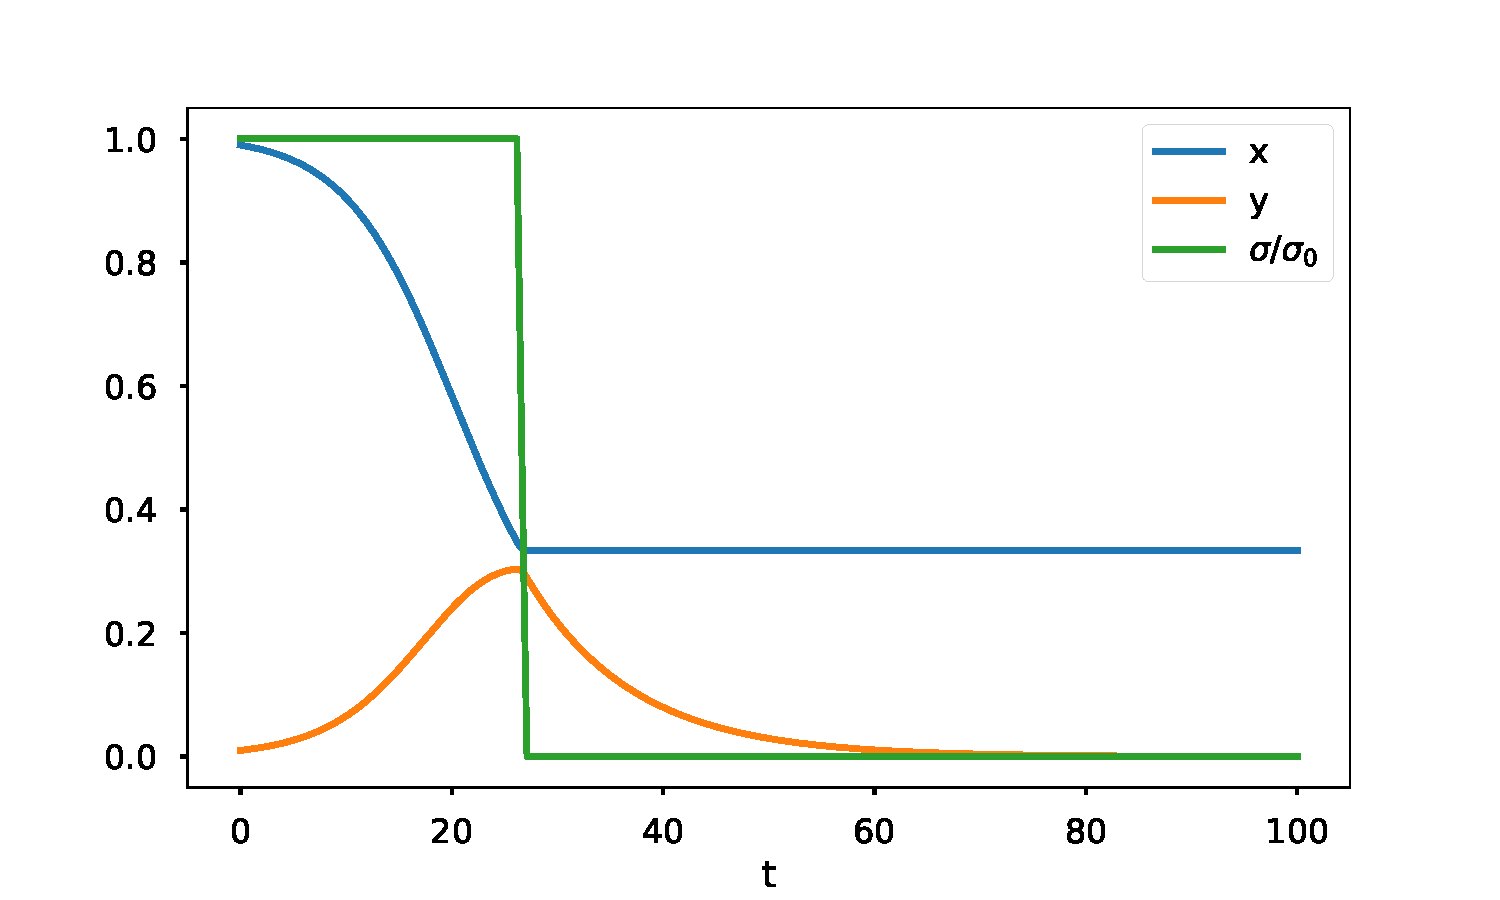
\includegraphics[width=0.65\textwidth]{figures/example1_time.pdf}}
    \subfigure[Trajectory in phase space]{\label{fig:ex1-xy}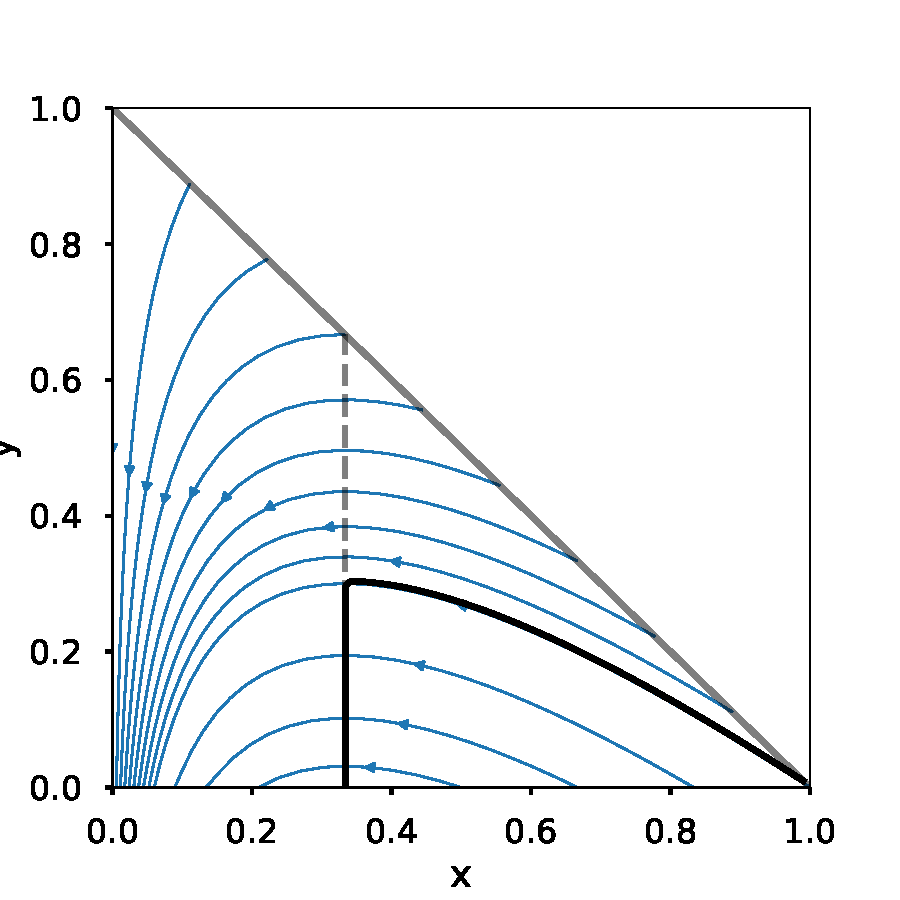
\includegraphics[width=0.34\textwidth]{figures/example1_xy.pdf}}
    \caption{Typical optimal solution.  Here $(x(0),y(0)) = (0.99,0.01)$, $\beta=0.3$, and $\gamma=0.1$.\label{fig:example1}}
\end{figure}

\begin{figure}
    \centering
    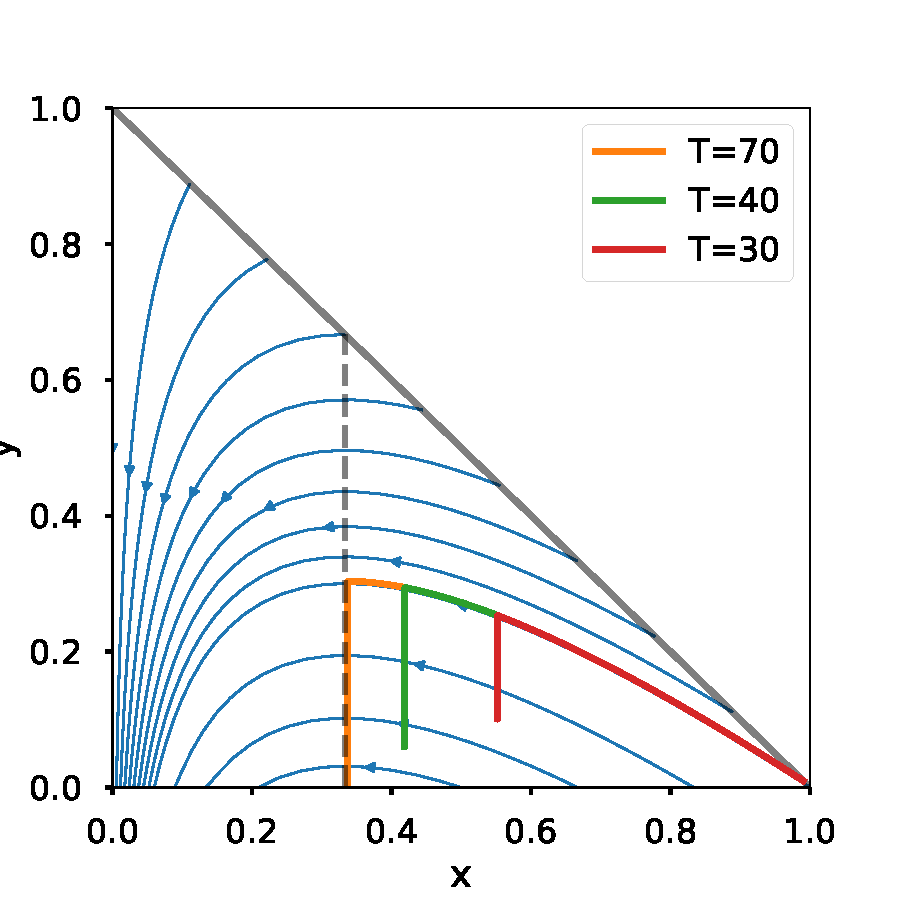
\includegraphics[width=0.5\textwidth]{figures/diff-time-opt.pdf}
    \caption{Optimal solutions starting from the same point $(0.99,0.01)$ but with different
        final times.  A larger value of $T$ allows the system to reach a more optimal state.
        For all solutions, $\beta=0.3$ and $\gamma=0.1$.\label{fig:diff-time-opt}}
\end{figure}

In real-world scenarios, it may not be possible to apply the maximum control $\sigma(t)=0$.
Suppose that in place of \eqref{q-shortterm} we impose $\sigma_\textup{min} \le \sigma(t) \le \Rnot$.
In this case the optimal control is still bang-bang with a single switching time.
In Figure \ref{fig:example_2}, we show an optimal solution when $\sigma(t)\ge 0.4\Rnot$ is imposed.

\begin{figure}
    \centering
    \subfigure[Solution and control vs. time]{\label{fig:example_2-t}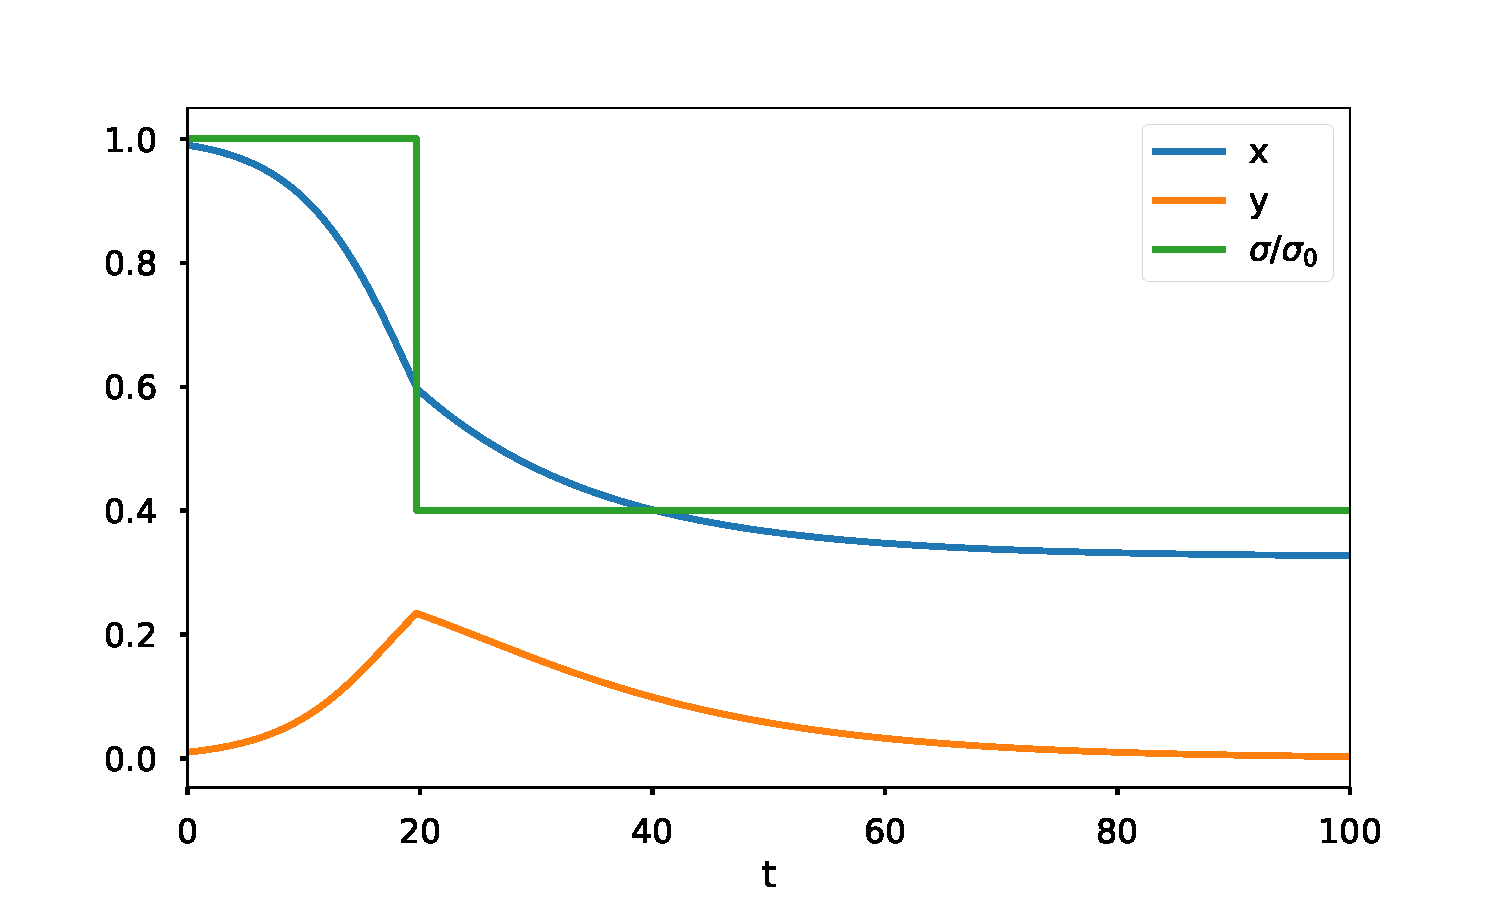
\includegraphics[width=0.65\textwidth]{figures/example2_time.pdf}}
    \subfigure[Trajectory in phase space]{\label{fig:example_2-xy}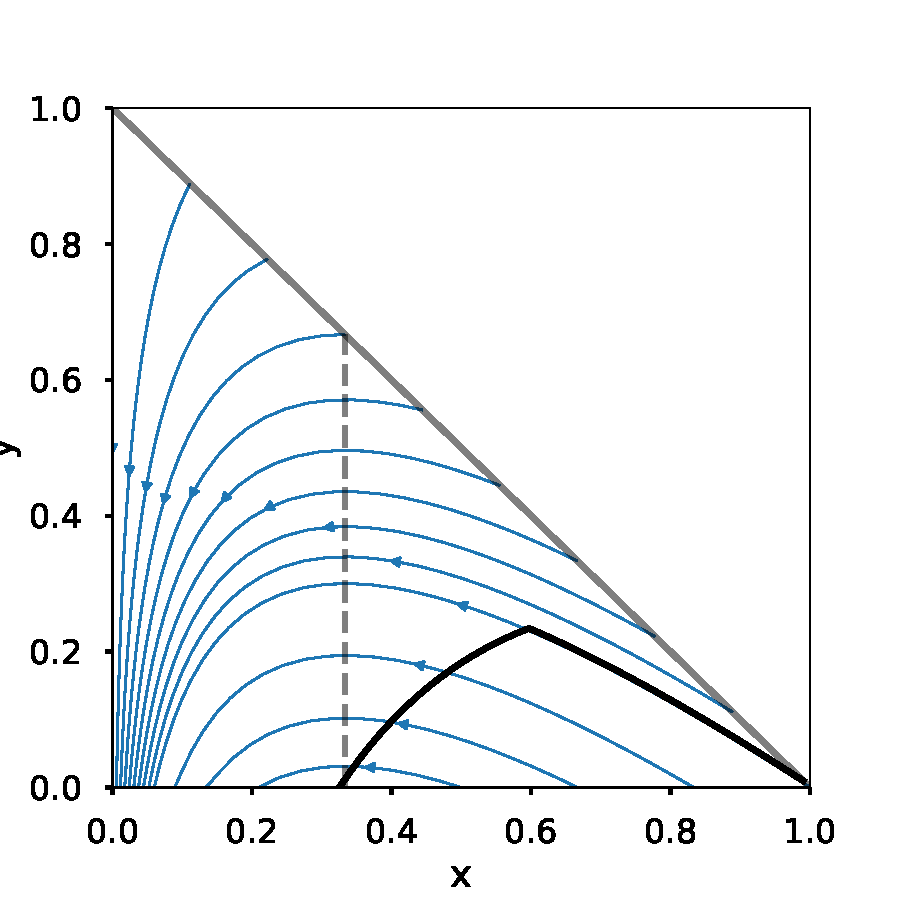
\includegraphics[width=0.34\textwidth]{figures/example2_xy.pdf}}
    \caption{Optimal solutions with $\sigma(t)\ge 0.4\Rnot$.  Here $(x(0),y(0)) = (0.99,0.01)$, $\beta=0.3$, $\gamma=0.1$, and $T=100$.\label{fig:example_2}}
\end{figure}

The switching time \eqref{xtstar} can also be derived via the Hamilton-Jacobi-Bellman (HJB) equation
for \eqref{eq:no-cost-problem}.  The HJB equation for $u(x,y,t)$ can be written
\begin{subequations} \label{eq:hjb-no-cost}
\begin{align}
    u_t & = \gamma y(t) u_y - \gamma x y \min_\sigma \left((u_y-u_x)\sigma\right) \\
    u(x,y,T) & = -\Sinf(x,y,\Rnot).
\end{align}
\end{subequations}
The required minimum is obtained by taking
\begin{align} \label{eq:hjb-control}
    \sigma(t) & = \begin{cases} 
        0 & u_y(x,y,t) > u_x(x,y,t) \\
        \Rnot & u_y(x,y,t)<u_x(x,y,t).
    \end{cases}
\end{align}
From \eqref{xinf-grad} we see that $u_y(x,y,T)>u_x(x,y,T)$ for all $(x,y)$.
Thus for small enough values of $T-t$, the solution of \eqref{eq:hjb-no-cost} satisfies
\begin{align*}
    u_t & = \gamma y(t) u_y(x,y,t).
\end{align*}
The solution of this hyperbolic PDE is
\begin{align*}
    u(x,y,t) & = u(x,ye^{-\gamma(T-t)},T) = -\Sinf(x,ye^{-\gamma(T-t)}).
\end{align*}
Thus
\begin{align*}
    u_x(x,y,t) & = -\frac{\partial \Sinf}{\partial y(t)} \left(1- \frac{1}{x(t)\Rnot}\right) \\
    u_y(x,y,t) & = -\frac{\partial \Sinf}{\partial y(t)} e^{-\gamma(T-t)}.
\end{align*}
According to \eqref{eq:hjb-control}, the optimal control value will switch when $u_x=u_y$, which
leads to \eqref{xtstar}.


\section{Optimal control with $L\ne 0$\label{sec:exploration}}
We now consider the case of a non-zero Lagrangian, which allows us to account for factors
like the economic cost of intervention or heightened risks caused by hospital
overflow.  We formulate the Hamiltion-Jacobi-Bellman (HJB) equation for this problem and
apply an upwind numerical method to compute approximate solutions.
The numerical solutions obtained via the HJB equation have also been checked in each case
against solutions of the BVP given in Section \ref{sec:pmp}, and found to
agree within numerical errors.


\subsection{Quadratic running cost of control}
We now attempt to account for the economic cost of intervention.  Quantification
of the cost of measures like closing schools and businesses is a challenging
problem in economic modeling, and well outside the scope of the present work.
Based on the general idea that both the cost and the marginal cost will increase
with the degree of contact reduction, we take for simplicity
$$
    L(x(t),y(t),\sigma(t)) = c_2 \left(1-\frac{\sigma(t)}{\Rnot}\right)^2.
$$
The HJB equation for \eqref{eq:basic-problem} is then
\begin{subequations} \label{eq:hjb-q-cost}
\begin{align} \label{eq:hjb-q-cost-pde}
    u_t - \gamma y(t) u_y & = - \min_{0\le \sigma\le \Rnot} \left((u_y-u_x)\gamma x(t) y(t) \sigma(t) + c_2 \left(1-\frac{\sigma(t)}{\Rnot}\right)^2 \right) \\
    u(x(t),y(t),T) & = -\Sinf(x(t),y(t),\Rnot).
\end{align}
\end{subequations}
The minimum in \eqref{eq:hjb-q-cost-pde} is obtained with
\begin{align} \label{eq:hjb-sigma}
    \sigma(t) & = \min\left(1,\max\left(0,\Rnot\left(1-\frac{\Rnot\gamma}{2c_2}x(t) y(t) (u_y-u_x)\right)\right)\right).
\end{align}
We approximate the solution of \eqref{eq:hjb-q-cost}-\eqref{eq:hjb-sigma} using the first-order
upwind finite difference method:
\begin{align}
\begin{split}
    u(x_i,y_j,t_n) \approx U^{n}_{ij} & = U^{n-1}_{ij} + \\
    & \Dt \left(\gamma x_i y_j \sigma(x_i, y_j, t) (D^\pm_y U^{n-1}_{ij} - D^-_x U^{n-1}_{ij}) 
        + c_2\left(1-\frac{\sigma(t)}{\Rnot}\right) - \gamma y_j D^\pm_y U^{n-1}_{ij}\right),
\end{split}
\end{align}
where
\begin{align*}
    D^+_x U_{ij} & = \frac{U_{ij}-U_{i-1,j}}{\Dx}, \\
    D^\pm_y U_{ij} & =
    \begin{cases}
        \frac{U_{ij}-U_{i,j-1}}{\Dy} & y'(t;x(t),y(t),\sigma(t))<0 \\
        \frac{U_{ij+1}-U_{i,j}}{\Dy} & y'(t;x(t),y(t),\sigma(t))>0,
    \end{cases}
\end{align*}
and $\sigma_{ij}(t)$ is given by a centered difference discretization of \eqref{eq:hjb-sigma}.
Note that the upwind $x$-direction is always to the left, since $x'(t)\le0$.

Numerical solutions for a range of values of $c_2$ are shown in Figure \ref{fig:varying_c2}.
The values of $c_2$ used here are chosen merely to illustrate the range of possible behaviors.
Notice that the strength of the control $\sigma(t)$ at early times varies non-monotonically
with $c_2$, first increasing and then decreasing as $c_2$ is reduced.  Indeed, the optimal
control $\sigma(t)$ over the initial time interval is simply $\Rnot$ in both limits $c_2 \to \infty$ and $c_2 \to 0$.

\begin{figure}
    \centering
    \subfigure[Solution (solid line) and control $\sigma(t)/\Rnot$ (dashed line) vs. time]{\label{fig:varying-c2}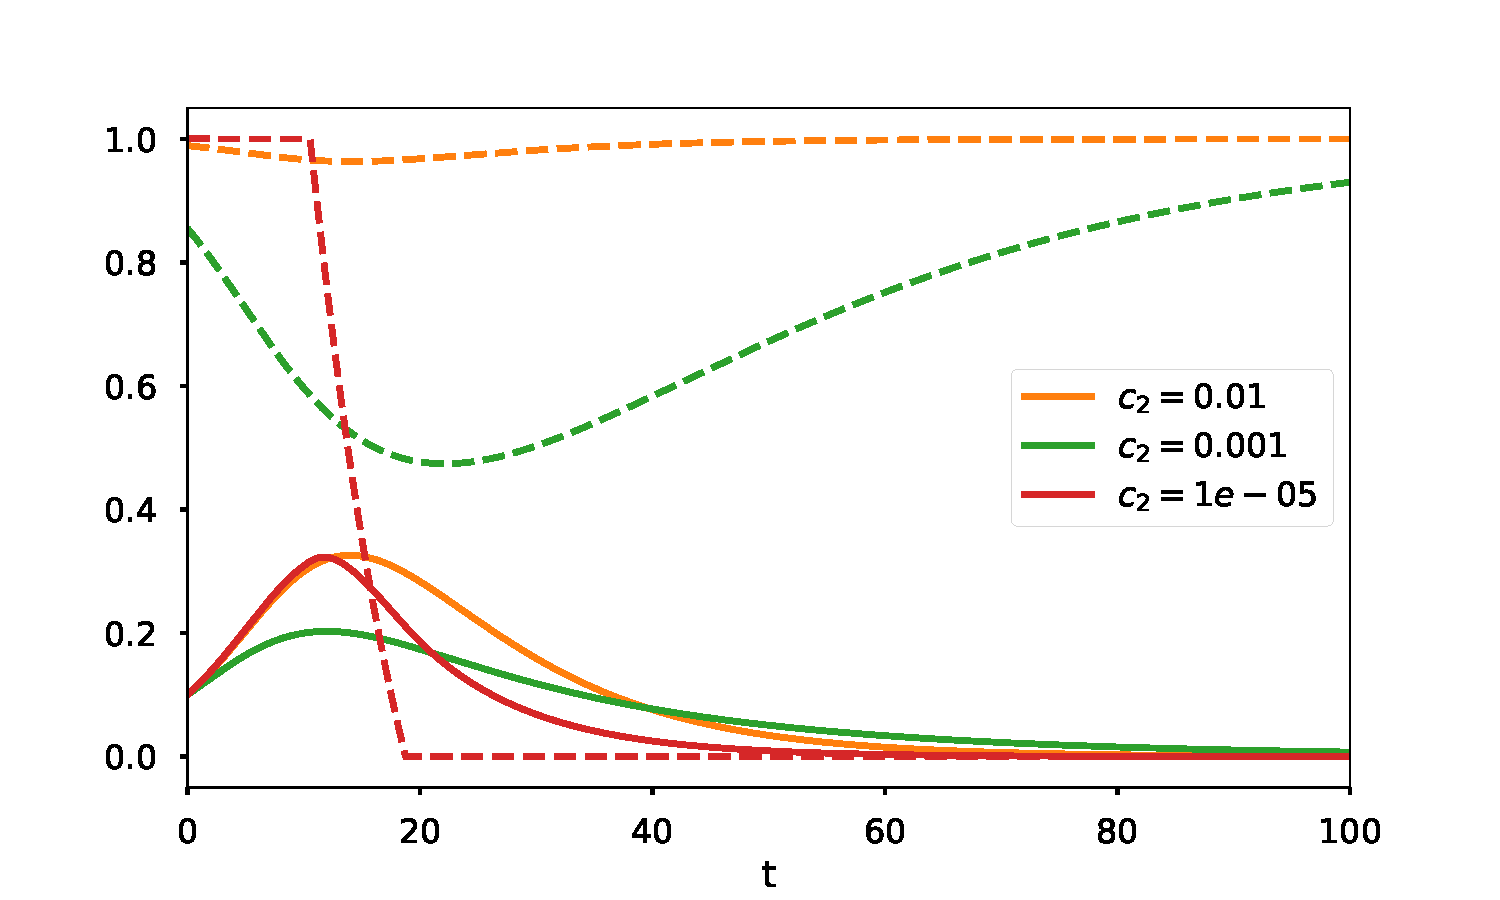
\includegraphics[width=0.65\textwidth]{figures/varying_c2.pdf}}
    \subfigure[Trajectory in phase space]{\label{fig:varying-cs-xy}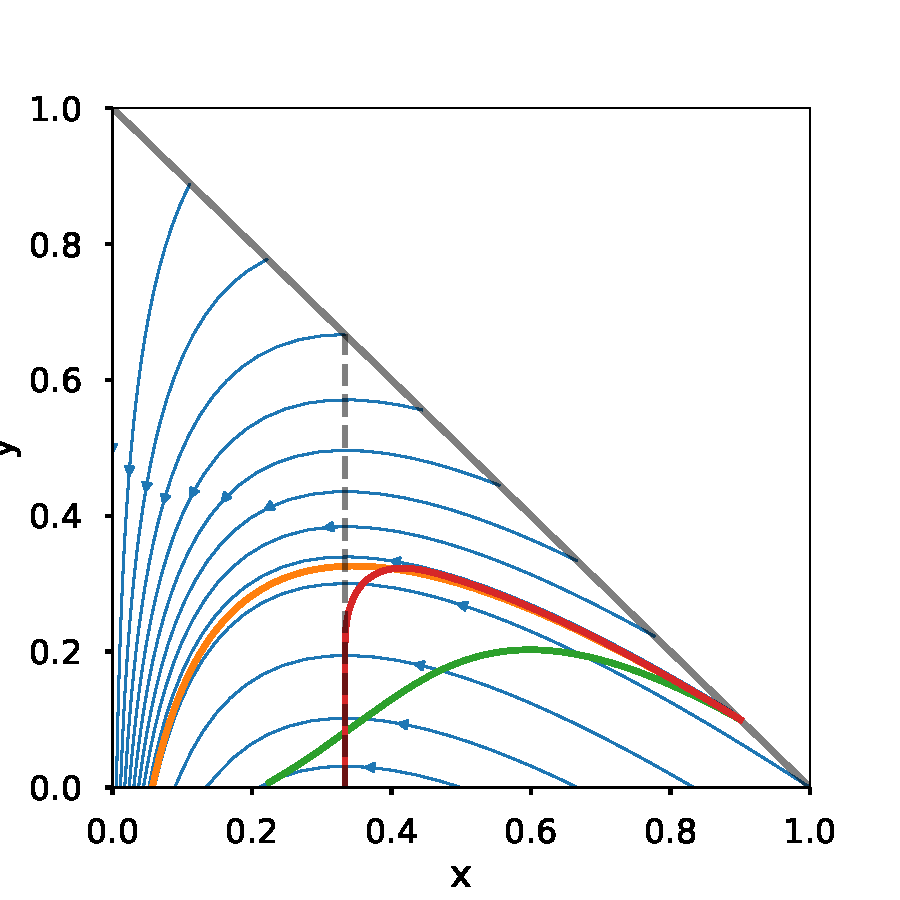
\includegraphics[width=0.34\textwidth]{figures/varying_c2_xy.pdf}}
    \caption{Optimal solutions with different running cost.  Here $(x(0),y(0)) = (0.99,0.01)$, $\beta=0.3$, $\gamma=0.1$, and $T=100$.\label{fig:varying_c2}}
\end{figure}


\subsection{Minimizing hospital overflow}
The optimal solutions above may be unsatisfactory in practice,
since the number of people simultaneously infected at certain times
may be too great for all of them to receive adequate medical care.  This is a major concern
with respect to the current COVID-19 crisis.  A natural objective is to keep
the number of infected below some threshold, corresponding for instance to the
number of hospital beds.  We thus consider the Lagrangian
$$
    L(x(t),y(t),\sigma(t)) = c_2 \left(1-\frac{\sigma(t)}{\Rnot}\right)^2 + c_3 g(y(t)-y_\text{max}).
$$
Here $\ymax$ is the maximum number of hospital beds.
The HJB equation is then
\begin{subequations} \label{eq:hjb-hosp}
\begin{align} \label{eq:hjb-hosp-pde}
    u_t - \gamma y(t) u_y - c_3 g(y(t)-y_\text{max}) & = - \min_{0\le \sigma\le \Rnot} \left((u_y-u_x)\gamma x(t) y(t) \sigma(t) + c_2 \left(1-\frac{\sigma(t)}{\Rnot}\right)^2 \right) \\
    u(x,y,T) & = -\Sinf(x(t),y(t),\Rnot).
\end{align}
\end{subequations}
The control that achieves the minimum in \eqref{eq:hjb-hosp-pde} is again given by \eqref{eq:hjb-sigma}.
The function $g(v)$ should be nearly zero for $v<0$ and increase
in an approximately linear fashion for $v>0$.  For the purpose of having
a tractable control problem, it is also desirable that $g$ be differentiable.
We take
$$
g(v) = \frac{v}{1+e^{-10v}}.
$$
Figures \ref{fig:min_hosp_1} and \ref{fig:min_hosp_2} show examples of solutions.
Again, we choose parameter values that demonstrate the range of qualitative behaviors.
In both examples, the cost of control is scaled by $c_2=10^{-3}$.
In Figure \ref{fig:min_hosp_1}, a higher cost for hospital overflow is applied,
with $c_3=10$).  As might be expected, $y(t)$ is generally
kept below $\ymax$ (which is set to $0.1$).
The control is initially off, then turns on
to avoid hospital overflow, and then turns off again.  While the control is applied,
it is maintained at a level that keeps the value of $y(t)$ nearly constant in time.

\begin{figure}
    \centering
    \subfigure[Solution and control vs. time]{\label{fig:minhosp1-time}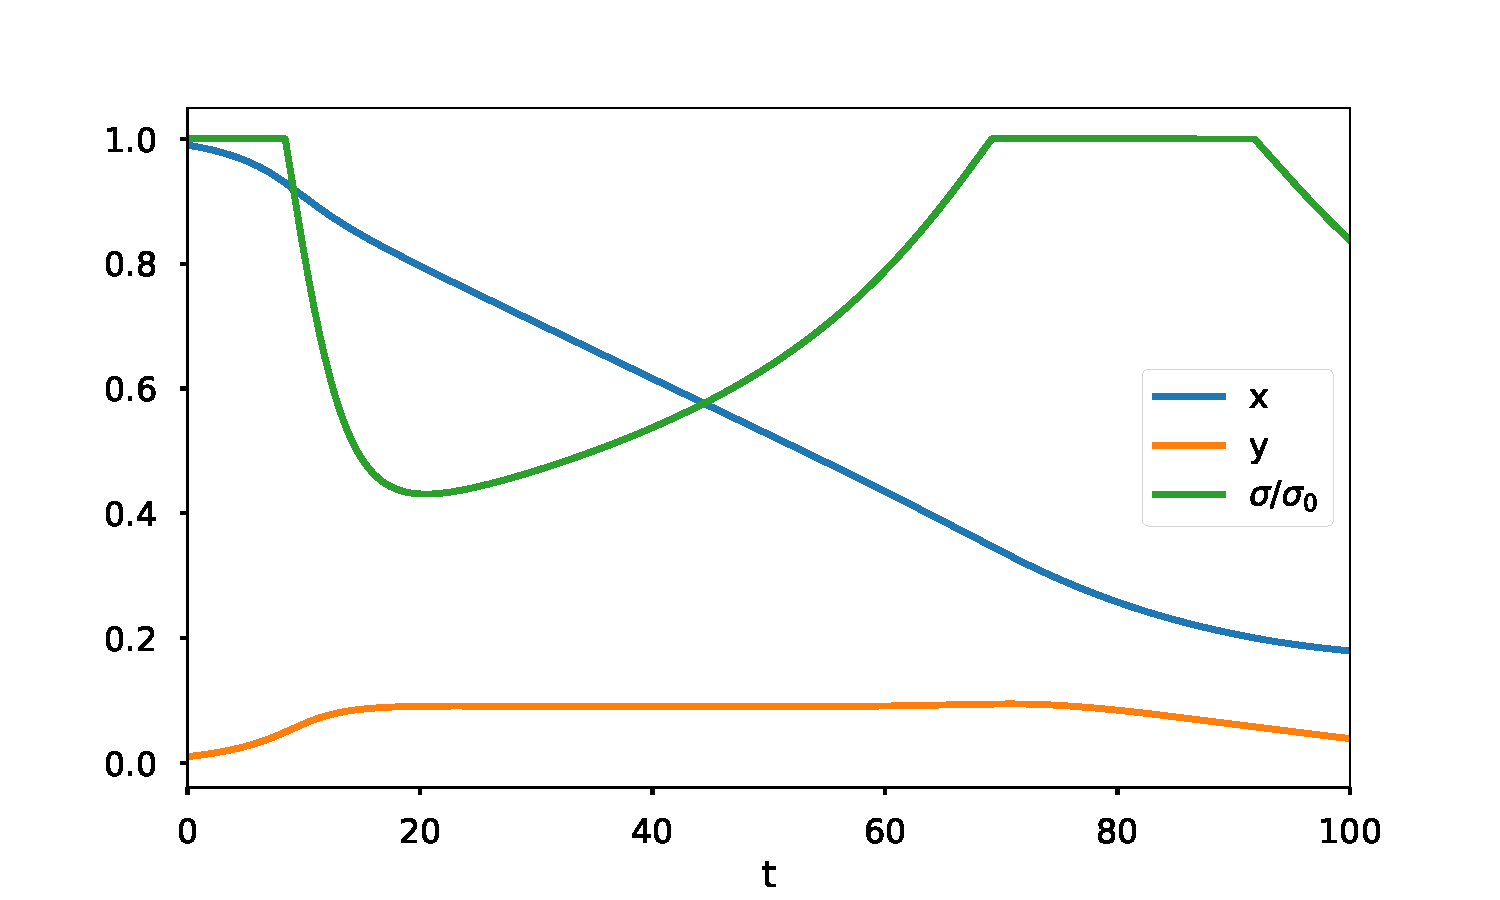
\includegraphics[width=0.65\textwidth]{figures/min_hosp_1_t.pdf}}
    \subfigure[Trajectory in phase space]{\label{fig:minhosp1-xy}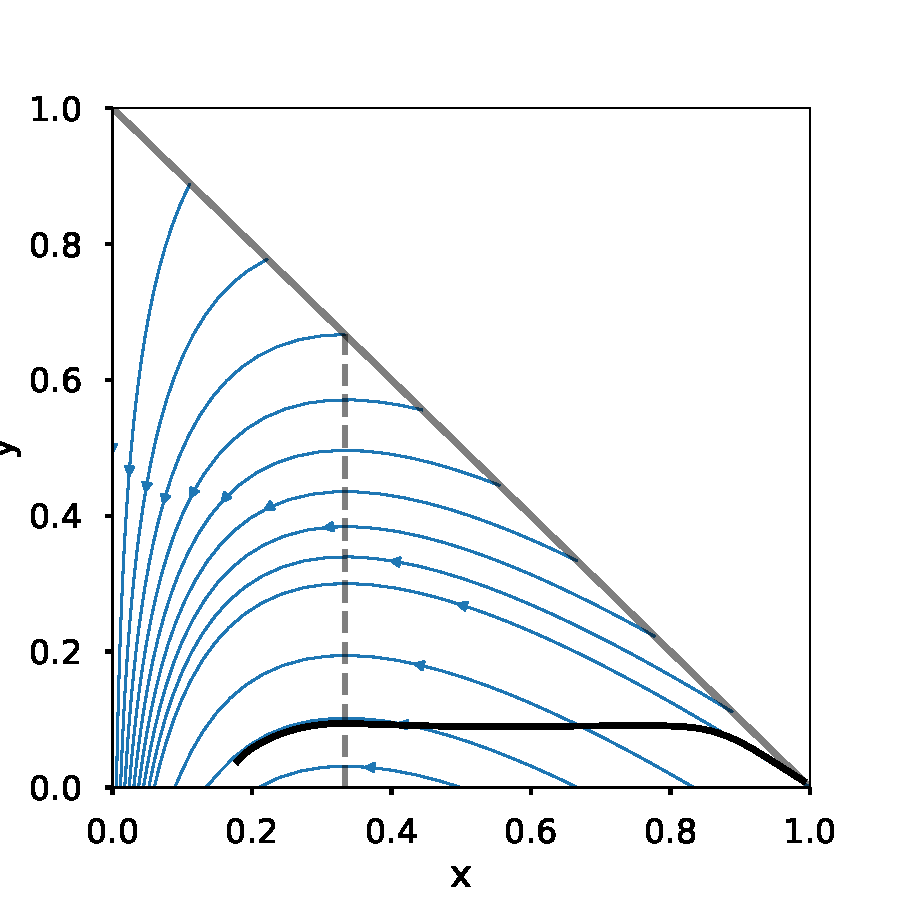
\includegraphics[width=0.34\textwidth]{figures/min_hosp_1_xy.pdf}}
    \caption{Optimal solutions with cost for hospital overflow.  Here $(x(0),y(0)) = (0.99,0.01)$, $\beta=0.3$, $\gamma=0.1$, $T=100$,
        and $\ymax=0.1$.
        In the cost function, we take $c_2=10^{-3}$ and $c_3=10$.\label{fig:min_hosp_1}}
\end{figure}

Figure \ref{fig:min_hosp_2} shows another example scenario in which the cost of hospital overflow is smaller,
with $c_3=10$.  In this case the hospital capacity is significantly exceeded for a short time.

\begin{figure}
    \centering
    \subfigure[Solution and control vs. time]{\label{fig:minhosp2-time}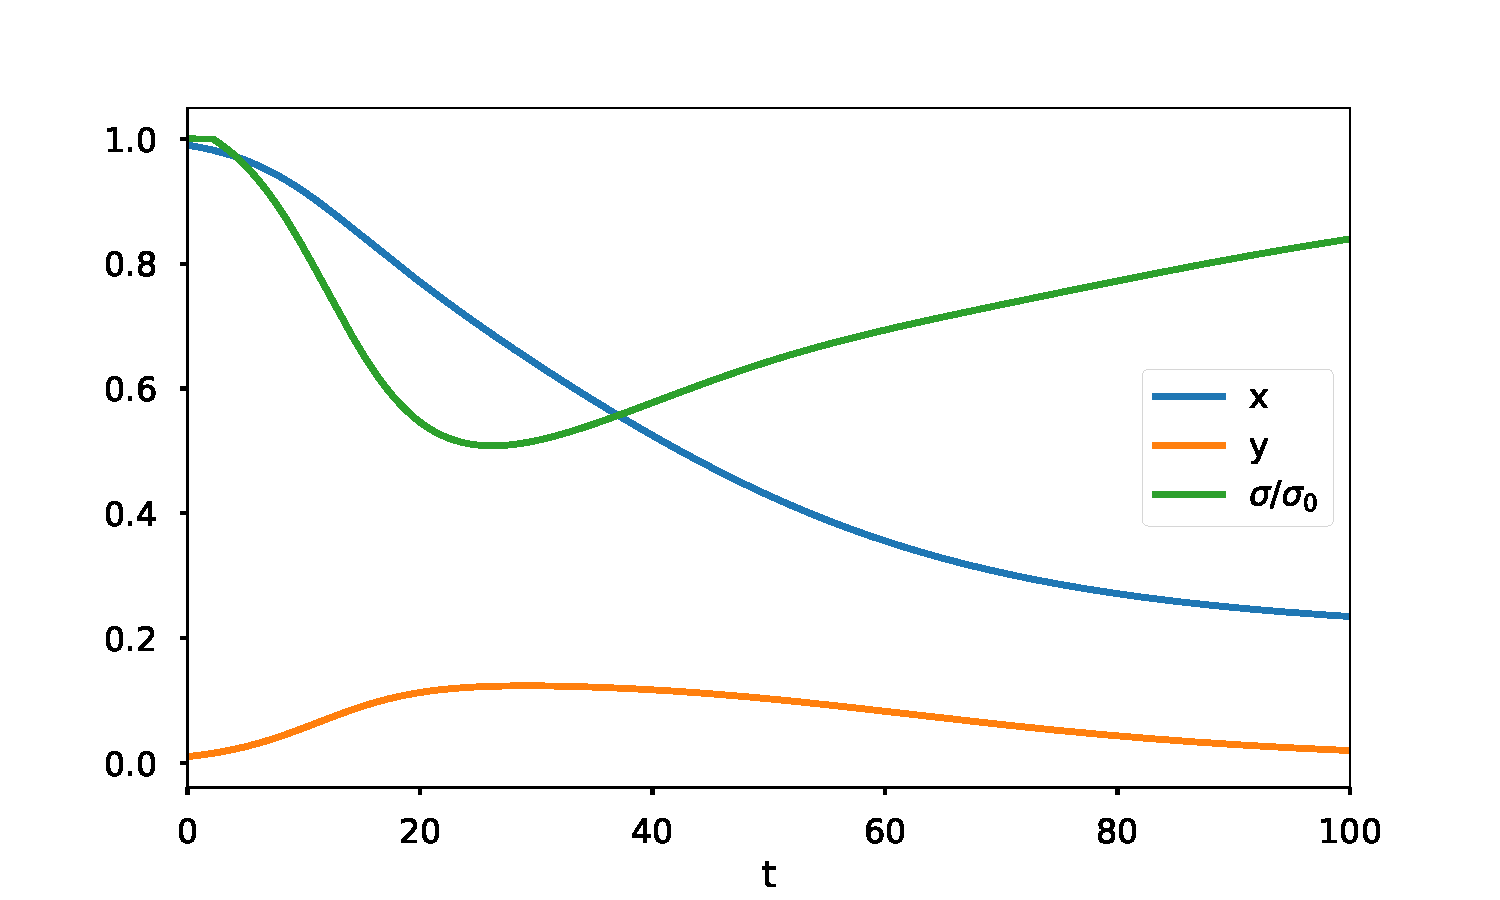
\includegraphics[width=0.65\textwidth]{figures/min_hosp_2_t.pdf}}
    \subfigure[Trajectory in phase space]{\label{fig:minhosp2-xy}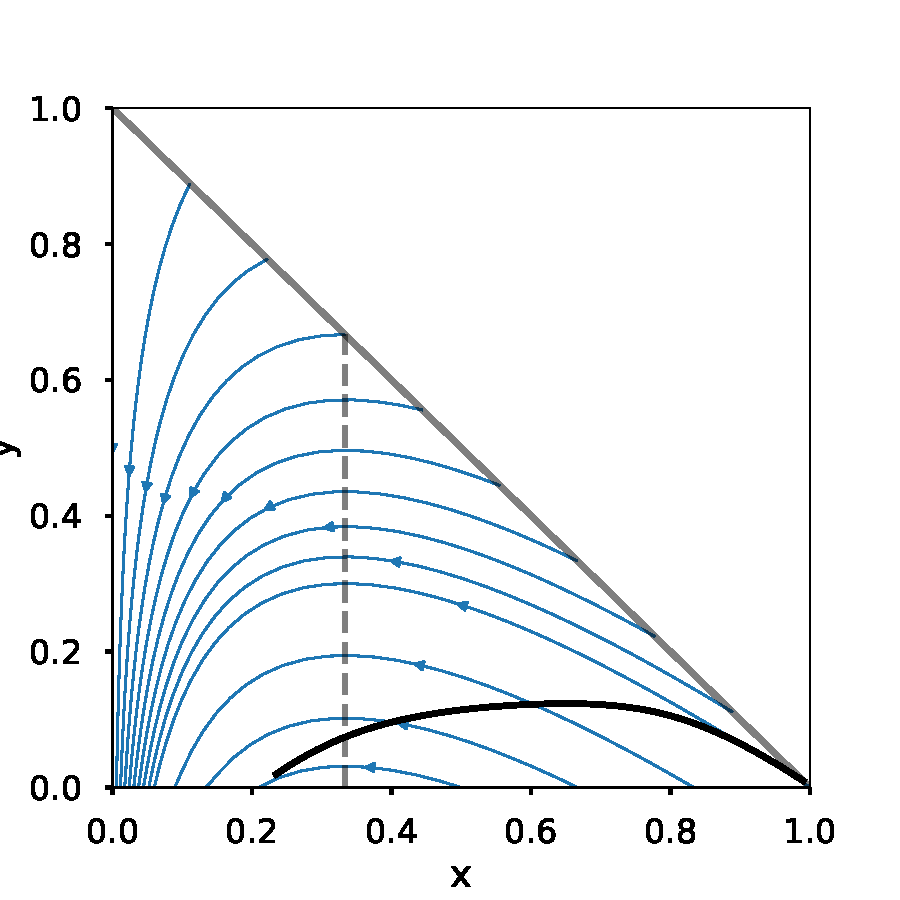
\includegraphics[width=0.34\textwidth]{figures/min_hosp_2_xy.pdf}}
    \caption{Optimal solutions with smaller cost for hospital overflow.  Here $(x(0),y(0)) = (0.99,0.01)$, $\beta=0.3$, $\gamma=0.1$, $T=100$,
        and $\ymax=0.1$.
        In the cost function, we take $c_2=10^{-3}$ and $c_3=1$.\label{fig:min_hosp_2}}
\end{figure}

\section{Application to the COVID-19 pandemic\label{sec:application}}
The main goal of this work has been a mathematical investigation of optimal
controls for the SIR model with a controlled rate of contact, as presented
in the previous sections.  We now present a brief illustration of the results
in practical terms through application to the current COVID-19 pandemic.
This application is imprecise, for several reasons:  the SIR model
is one of the simplest epidemiological models, and assumes homogeneous mixing
among a population; the current state of susceptible and infected persons is
not accurately known; and the parameters of the disease itself (i.e. $\gamma, \Rnot$)
are still quite uncertain.  
%Finally, and perhaps most importantly, we have
%at present little data with which to quantify the effect of current interventions,
%and we cannot predict the course of future intervention policies.
The examples in this section should be viewed only as illustrations
of a few possible scenarios, and not an exhaustive or detailed study.

We take the infectious period $\gamma^{-1}=10$ days, and the basic reproduction
number $\Rnot=2.5$, based on recent estimates \cite{verity2020estimates,liu2020reproductive}.
To make the results easy to interpret, we use a
fixed terminal cost of $c_1 z_\infty$, where we have introduced an additional
scaling constant.  Taking $c_1 = \alpha N$, where $N$ is the total population
being modeled and $\alpha$ is the infection fatality ratio, then this cost is
the expected number of lives lost.  Since $z_\infty=1-\Sinf$, this is merely a
rescaling of the terminal cost used throughout this work.  We take
$\alpha \approx 0.006$ based on recent estimates \cite{verity2020estimates,russell2020estimating,wu2020estimating}.

We seek reasonable order-of-magnitude estimates for $c_2$ and $c_3$.  
The value of $c_3/N$ should be equal to the increase in probability of a given
infected person dying because of the lack of medical care.  We take
$c_3 = N\eta$,
where the fatality ratio in the absence of medical care is $\alpha+\eta$.
In the absence of any relevant data, we take $\eta\approx 2\alpha$, giving
$c_3 = 0.0012N$.  For $\ymax$ we take values from the United States, where
there are about 3 hospital beds per 1000 people, and two-thirds of them
are typically occupied.  Since it is estimated that about 5\% of COVID-19
cases are hospitalized \cite{verity2020estimates}, this gives $\ymax=0.02N$.

Any attempt to quantify the cost of an intervention in human lives is bound
to be contentious.  Whether we consider the value of a human life to be in
intrinsic personal value or extrinsic economic value, we can view the cost
of intervention as a reduction of the value of human lives during the intervention
period.  We take $c_2 = N\epsilon/d$ where $d\approx 10^4$ is the number
of days in a human life (more precisely, the average number of days remaining
in a life claimed by the disease) and $1-\epsilon$ is the relative value of a
day spent in full isolation ($\sigma=0$) compared to a day without intervention.
Taking $\epsilon=0.2$, we have $c_2 = 2\times10^{-5} N$.

Since all terms in the cost function are proportional to $N$, we take $N=1$ without
loss of generality.  Results for the parameter values given above are shown in Figure
\ref{fig:real-world-1}.  We see that the optimal control corresponds to a level
of intervention that becomes more strict as the epidemic grows, and is gradually
relaxed as the epidemic subsides.  Most importantly, and in agreement with results
from the examples in earlier sections, the strongest control is applied around
the time of peak infection and shortly thereafter.
The maximum hospital capacity is significantly exceed, with the maximum value of $y$
around $0.08$.  This level of infection may still be manageable with local surges
of care facilities and staff, like those that have already been carried out in practice.
There is also a noticeable (but greatly reduced relative to the uncontrolled case)
epidemiological overshoot.

\begin{figure}
    \centering
    \subfigure[Solution and control vs. time]{\label{fig:real_world_1-time}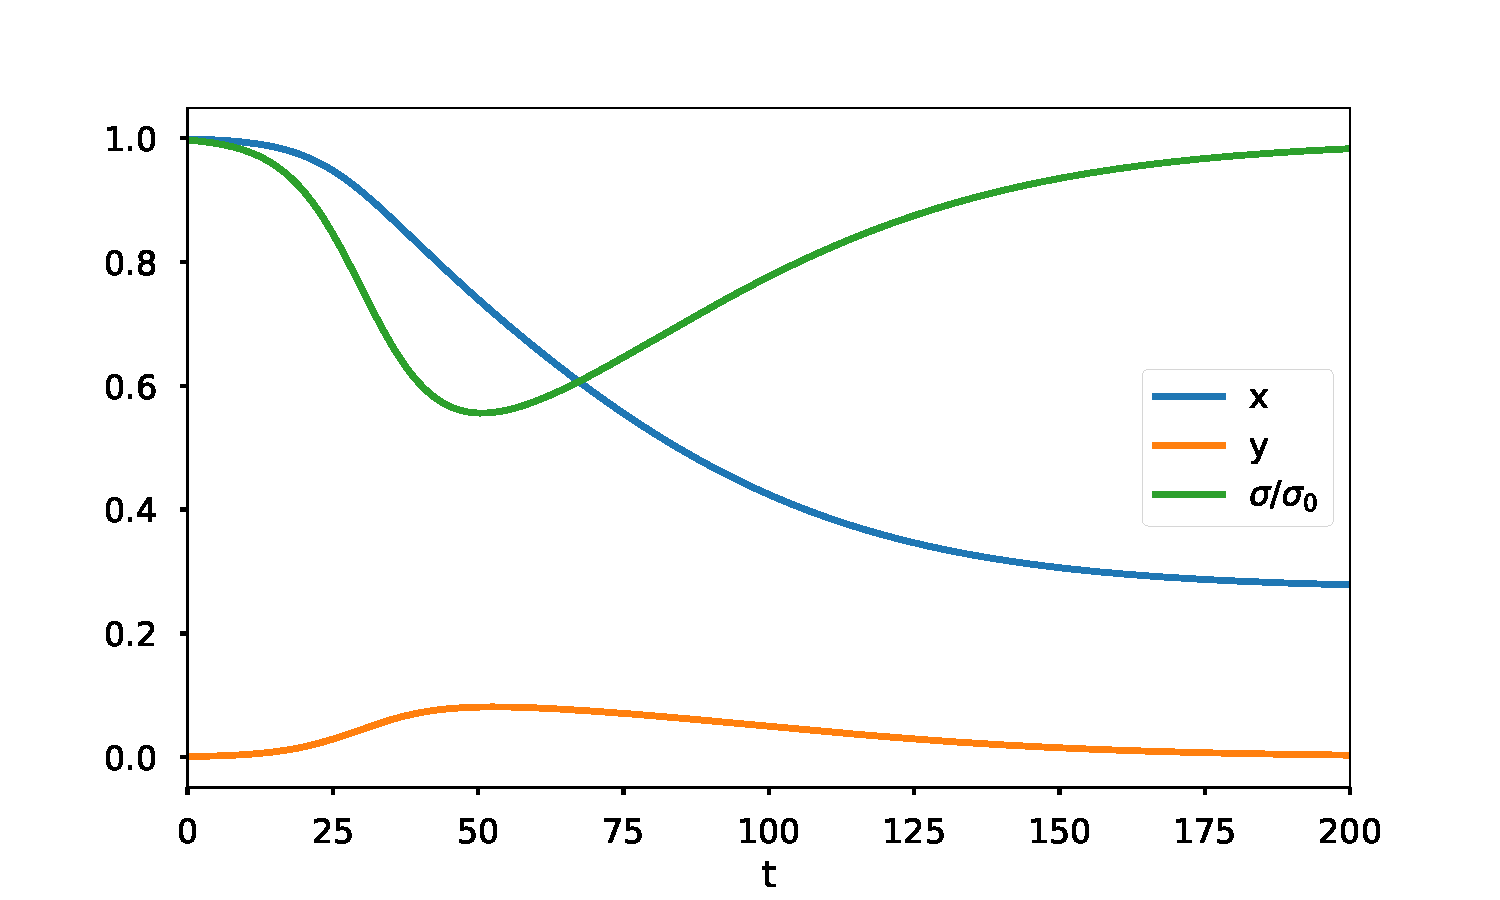
\includegraphics[width=0.65\textwidth]{figures/real_world_1_t.pdf}}
    \subfigure[Trajectory in phase space]{\label{fig:real_world_1-xy}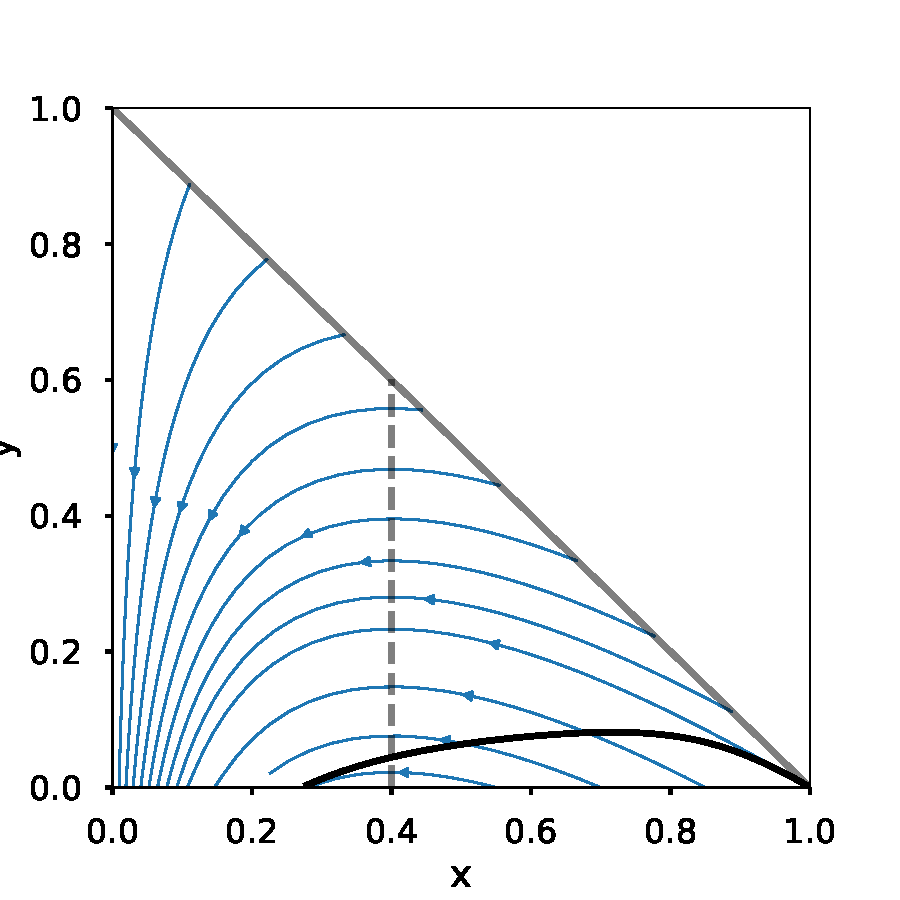
\includegraphics[width=0.34\textwidth]{figures/real_world_1_xy.pdf}}
    \caption{Optimal control for COVID-19 with $\Rnot=2.5$, $\gamma=0.1$,
                $\alpha=0.006$, $\eta=0.012$, $\epsilon=0.2$, $d=10^4$, $T=200$, and $(x(0),y(0)) =
                (0.999,0.001)$.\label{fig:real-world-1}}
\end{figure}

An alternative scenario is shown in Figure \ref{fig:real-world-2}, in which
we have assumed a fatality ratio and a value of $\eta$ that are twice as
large (in line with the highest estimates of the infection fatality ratio),
as well as taking $\epsilon=0.05$.  These parameters lead to stronger control,
especially in the later phases of the epidemic.
The result is a significant reduction in epidemiological overshoot and in
maximum infected (around $0.06$).

\begin{figure}
    \centering
    \subfigure[Solution and control vs. time]{\label{fig:real_world_2-time}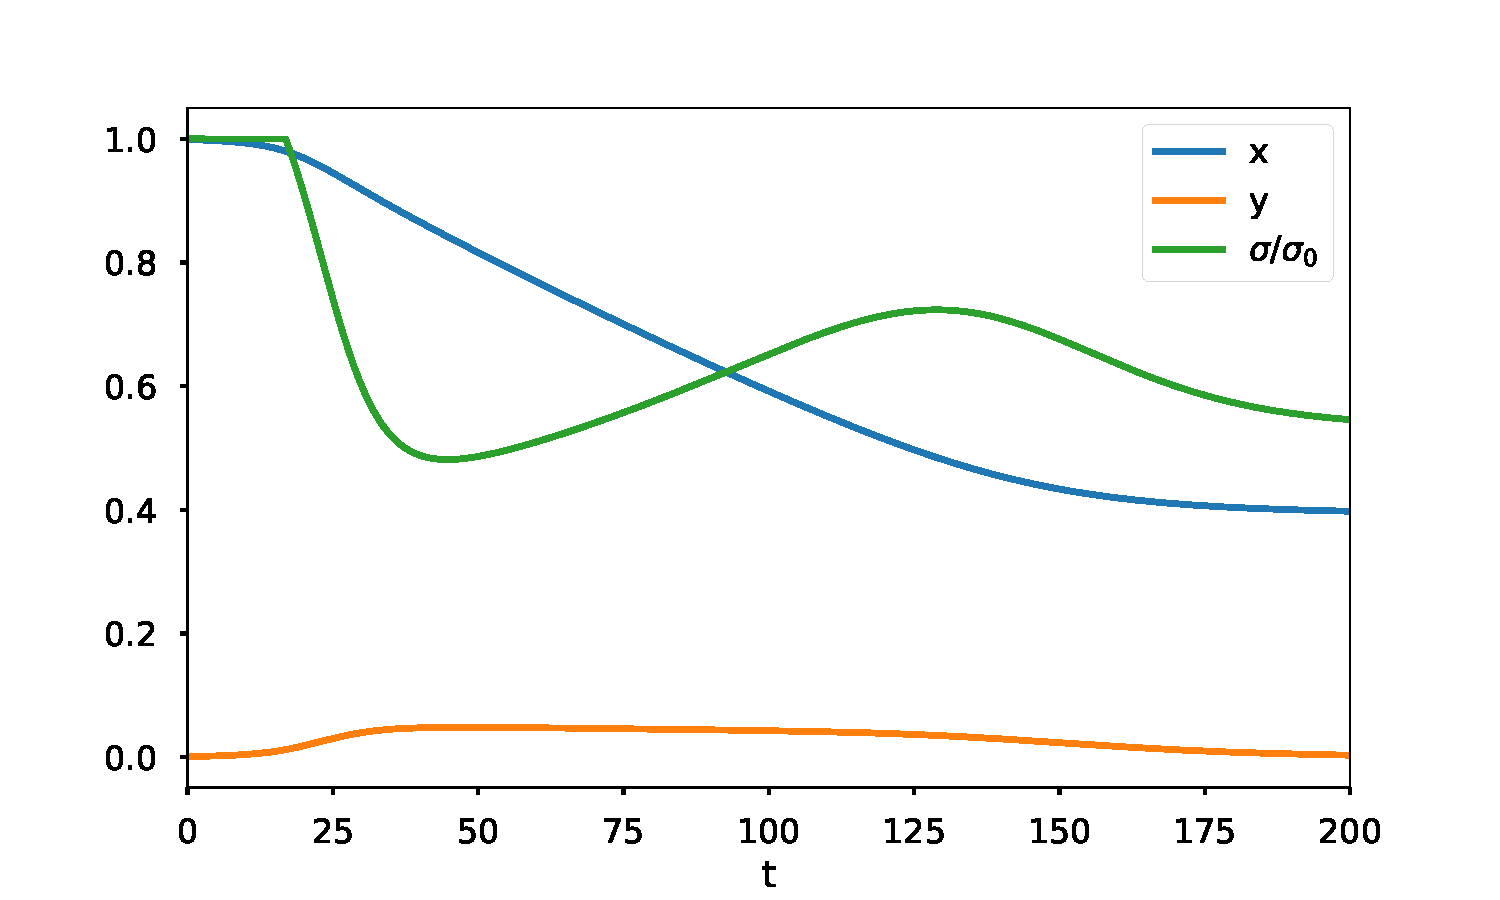
\includegraphics[width=0.65\textwidth]{figures/real_world_2_t.pdf}}
    \subfigure[Trajectory in phase space]{\label{fig:real_world_2-xy}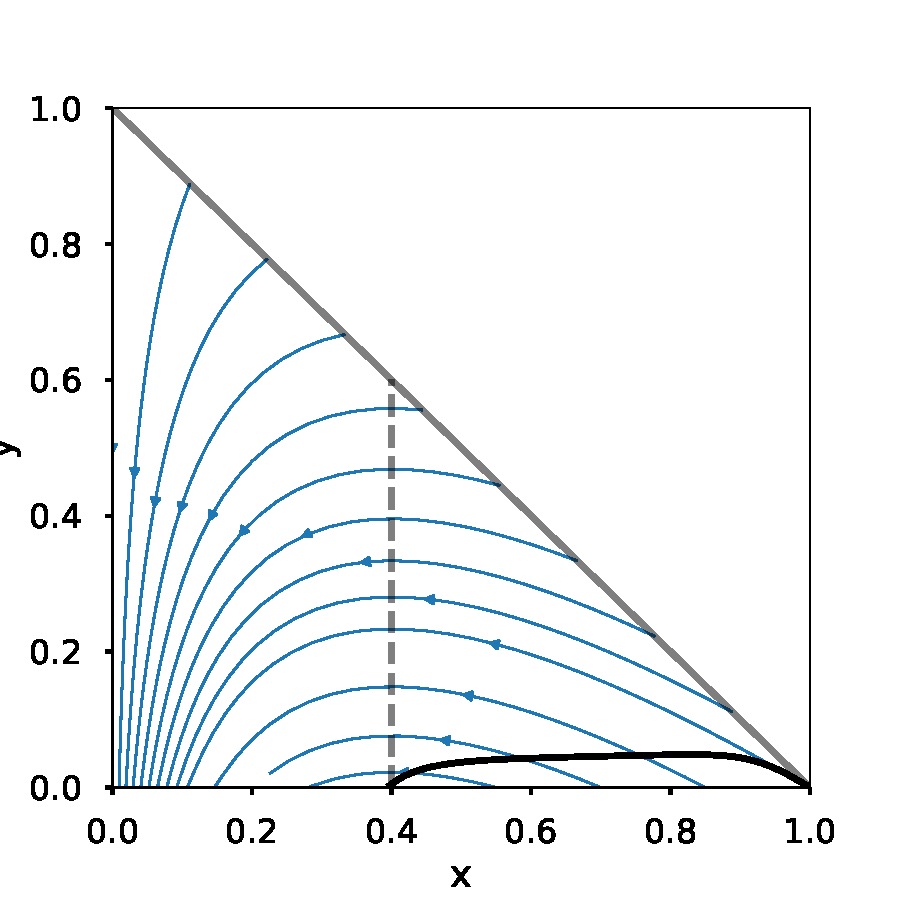
\includegraphics[width=0.34\textwidth]{figures/real_world_2_xy.pdf}}
    \caption{Optimal control for COVID-19 with $\Rnot=2.5$, $\gamma=0.1$,
                $\alpha=0.012$, $\eta=0.024$, $\epsilon=0.05$, $d=10^4$, $T=200$, and $(x(0),y(0)) =
                (0.999,0.001)$.\label{fig:real-world-2}}
\end{figure}

Finally, in Figure \ref{fig:real-world-3}, we repeat the first scenario
but increase the cost of control by taking $\epsilon=0.5$.
In this case a more mild control is applied, peaking at about
20\% contact reduction and concentrated around the time of the
infection peak.
\begin{figure}
    \centering
    \subfigure[Solution and control vs. time]{\label{fig:real_world_3-time}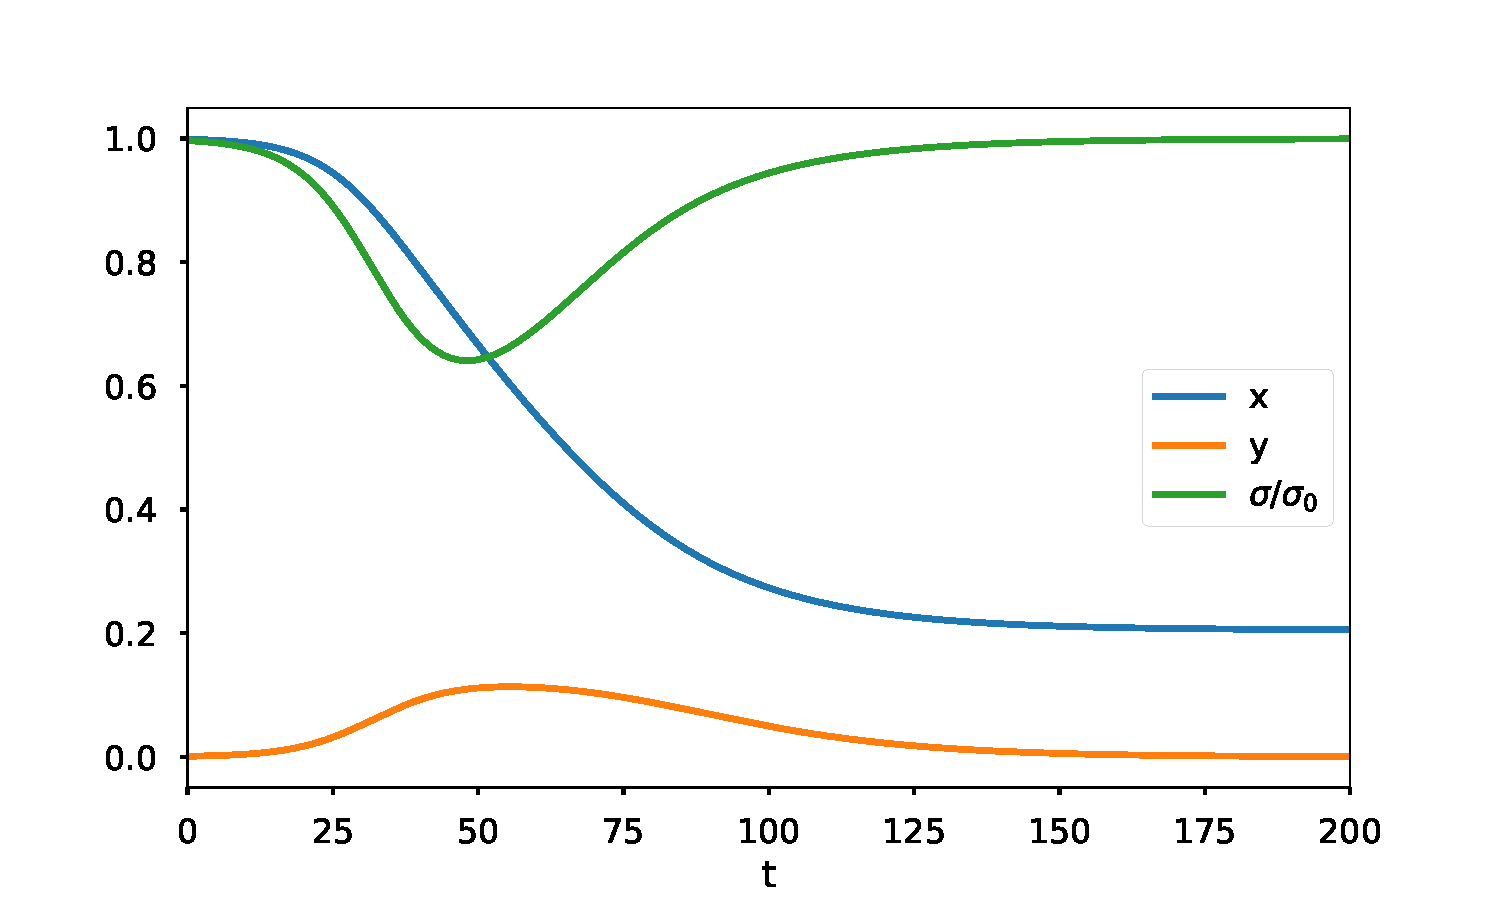
\includegraphics[width=0.65\textwidth]{figures/real_world_3_t.pdf}}
    \subfigure[Trajectory in phase space]{\label{fig:real_world_3-xy}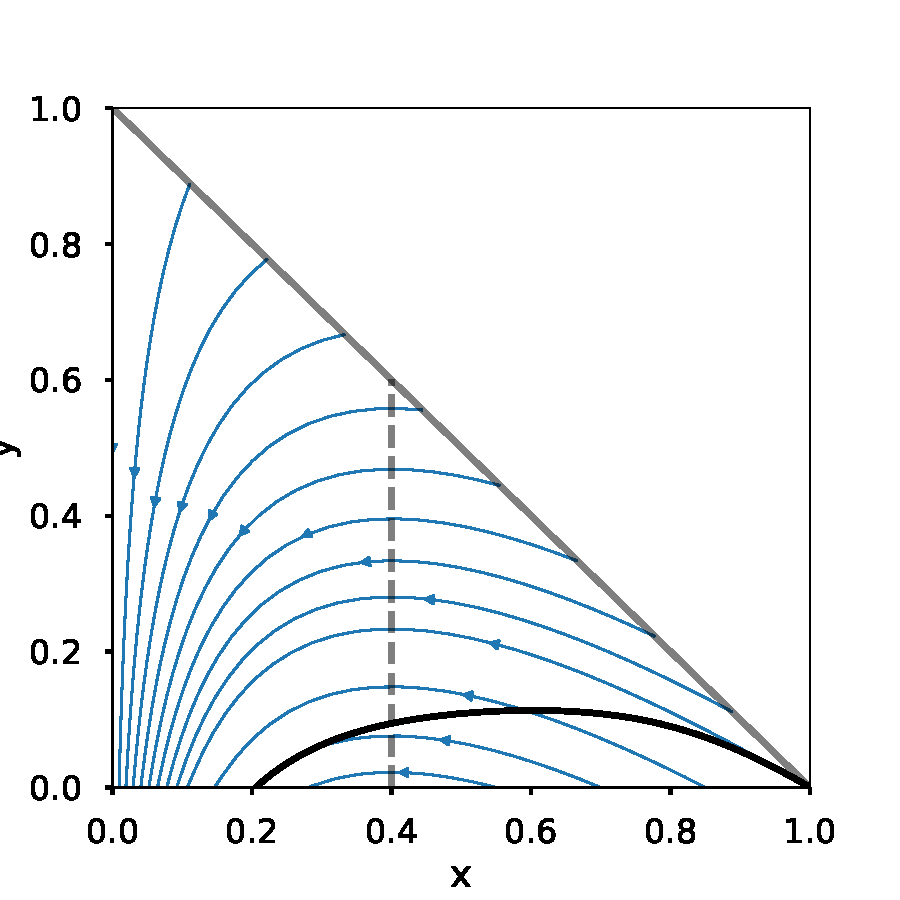
\includegraphics[width=0.34\textwidth]{figures/real_world_3_xy.pdf}}
    \caption{Optimal control for COVID-19 with $\Rnot=2.5$, $\gamma=0.1$,
                $\alpha=\eta=0.006$, $\epsilon=0.5$, $d=10^4$, $T=2000$, and $(x(0),y(0)) =
                (0.999,0.001)$.\label{fig:real-world-3}}
\end{figure}


\section{Conclusion\label{sec:conclusion}}
We have studied, for an SIR model with a control on the rate of contact, the
problem of minimizing the eventually infected population in the long-time limit,
when the control can be applied only up to a finite time.  In the absence of any
cost of intervention, the optimal strategy is to apply no control until a
certain switching time, and then apply maximum control.  We have also considered
other objective functions that include a running cost of control and a penalty for
large numbers of simultaneous infections.

A common feature of all solutions is that the optimal control is strongest around
the time of peak infection.  This is because the payoff for contact reduction
is larger when the infected population is larger.
The idea that intervention should possibly be delayed in order to increase
its effect was also found in \cite{ballard2017intervention}, although 
the objective and optimal policy found there differ from the present work.

Although this work has focused on fundamental mathematical theory, there are
important implications that are relevant to real-world epidemics.  First,
observe that the optimal solutions obtained here, based on maximizing $\Sinf$, are
drastically different than those that would be obtained if the objective
were to maximize $x(T)$ (which would make sense, for instance, if it were
expected that a vaccine would be available at time $T$).  In the latter case, an optimal strategy over
short times may be to apply very strong control from the outset.  But the long-term
outcome of such a strategy, if intervention cannot be maintained forever,
and in the absence of a vaccine, is simply to delay the epidemic.  This has
been borne out in real epidemics.
A study of the 1918 influenza pandemic found no statistically significant
correlation between interventions and the eventual death toll in US cities
\cite{hatchett2007public}.  In simple terms, flattening the curve also
broadens the curve and may not have a substantial impact on the area under the
curve, especially if the level of control is relaxed as soon as the
number of infections starts to decrease.

Real-world application of the strategies derived here would require
precise knowledge of the disease parameters, the current state of the
population, and the quantitative effect of specific NPIs, none of which
are readily available (or indeed capable of being characterized by a single
number).  Nevertheless, the general results obtained here may provide insight
into what optimal intervention strategies and their consequences may look like.


\bibliographystyle{plain}
\bibliography{refs}

\end{document}
